\chapter{Efficiency evaluation}
\label{chap:prod:effs}

The efficiency chain defines the fraction of prompt charm mesons that survive
the full reconstruction and selection procedure within each \pTy\ bin.
The chain is defined in steps grouped by physical requirements and those
imposed by software, with each step being relative to the previous one.
This starts with the efficiency of a signal charm hadron to decay within the
\lhcb\ acceptance having been produced in a \pp\ collision, \effacc.
The efficiency of such a decay to be fully reconstructed is the reconstruction
efficiency \effreco, and then the efficiency of the reconstructed decay to
be triggered through \lzero, \hltone, and \hlttwo\ is the trigger efficiency
\efftrig.
There is also the efficiency of triggered candidates to pass through the
offline selection \effoffline, and finally there is the signal window
efficiency \effsigwin\ due to the requirement imposed before the \lnipchisq\
fit.
The total efficiency, \eff, is the product of these, and is what enters in
\cref{eqn:prod:introduction:differential_cross_section}.

Two methods are used for efficiency estimation: with simulation, where
true information is available before and after all steps; and methods of
calibration, where proxy data selected without the use of particular
information can be used to assess the effects of using that information in the
analysis data.
Efficiency evaluation with \ac{MC} can be simple, but differences between the
data and the \ac{MC} must be accounted for.
Calibration techniques use real data, and so can be more robust than \ac{MC},
but obtaining clean calibration samples can be challenging.

In \lhcb, it is known that the \ac{PID} selection efficiencies are not
well-modelled in the \ac{MC} due to an under-estimation of the detector
occupancies.
The same is true, albeit to a lesser extent, for the reconstruction
efficiencies.
Kinematic variables, such as charm hadron and final-state momenta, are
comparatively well-modelled.
This motivates a two-step procedure for evaluating the \emph{selection}
efficiency, whereby the \ac{PID} efficiency is computed using calibration
techniques, described in \cref{chap:prod:effs:pid}, and the efficiency of the remaining
requirements is made using \ac{MC}, detailed in \cref{chap:prod:effs:sel}.
The reconstruction efficiency will be computed using \ac{MC}, but corrected
with a factor obtained from calibration samples, described in \cref{chap:prod:effs:acc}.
The extent to which these techniques do not accurately model the efficiencies
will be discussed in the context of systematic uncertainties in
\cref{chap:prod:syst:mc}.

The matching of true \ac{MC} particles to reconstructed objects, the process of
truth-matching as described in \cref{chap:prod:data:mc}, is not \SI{100}{\%}
efficient, and so a correction factor \efftruth\ is computed to account for
the deficit.

To summarise: the total efficiency $\eff_{i}(\decay{\PHc}{f})$, for charm
candidates in the $i$th \pTy\ bin, is the product of the individual
efficiencies and correction factors
\begin{align}
  \eff_{i}(\decay{\PHc}{f}) = \effacc &\times \effreco \times \efftruth \times \efftracking \nonumber\\
                                      &\times \efftrig \times \effoffline \times \effpid \times \effsigwin.
  \label{eqn:prod:effs:total_eff}
\end{align}
where each efficiency \eff\ is dependent on the charm hadron \PHc\ and the
final state $f$, and is conditional on the previous step.

In this \lcnamecref{chap:prod:effs} the details of the efficiency computation
for each step are given.
Example efficiency tables, differential in \pTy, for the
two-body \DzToKpi\ and three-body \DpToKpipi\ decays are given in
\cref{chap:app:production_tables}.
The notation for conditional yields will be used throughout, where $N_{B|A}$
denotes the prompt signal yield after process $B$ given that process $A$
preceded $B$.

\section{Detector acceptance}
\label{chap:prod:effs:acc}

The acceptance efficiency, evaluated using simulation, is due to the finite
spatial acceptance of the \lhcb\ detector.
The acceptance is modelled by a set of cuts requiring that all stable charged
particles in the final state have a momentum direction satisfying $10 < \theta
< \SI{400}{\milli\radian}$, and that all the particles in the final state point
in the positive $z$ direction.
These requirements are applied at the generator level, before the detector
simulation, on the true kinematics of the particles.

By counting the number of prompt charm hadrons passing the cut, the acceptance
efficiency is defined as
\begin{equation}
  \effacc = \frac{%
    N_{\text{Accepted}|\text{Generated}}
  }
  {%
    N_{\text{\text{Generated}}}
  }.
  \label{eqn:prod:effs:acc}
\end{equation}
The input dataset to this computation is the generator-level set described in
\cref{chap:prod:data:mc}.
The acceptance efficiencies for \DzToKpi\ and \DpToKpipi, in \pTy\ bins, are
given in \cref{tab:prod:effs:acc:dztokpi,tab:prod:effs:acc:dptokpipi}.

\section{Reconstruction}
\label{chap:prod:effs:reco}

The reconstruction efficiency \effreco\ parameterises the fraction of charm
meson decays passing the acceptance requirements that are also fully
reconstructed as tracks, for the final-state particles, and vertices, for the
charm mesons.
This folds in several effects: whether the final-state particles have a large
enough momentum not to be bent out of the detector acceptance by the magnetic
field; whether the final-state particles leave enough hits in the tracking
system to be reconstructible (that is, above the minimum threshold at which the
tracking system \emph{could} reconstruct a track); whether, given that enough
hits were deposited by a final-state particle, a track was actually
reconstructed; and whether a vertex can be formed, given that all final-state
particles have associated tracks.

The reconstruction efficiency is defined as the ratio of fully reconstructed
decays to those passing the acceptance requirements
\begin{equation}
  \effreco = \frac{%
    N_{\text{Reconstructed}|\text{Accepted}}
  }
  {%
    N_{\text{\text{Accepted}}}
  }.
  \label{eqn:prod:effs:reco}
\end{equation}
This definition is subject to the effects of \pTy\ bin `migration', whereby 
mesons are reconstructed as belonging to bins different from those of the true 
particles.
These can be due to resolution as well as any possible biases on the 
measurements of \pT\ and \rapidity.
If the net migration between bins is large, that is if the migrations are not 
symmetric, then the detector effects should be corrected for such that the 
reconstructed meson kinematics are more accurate estimators of their true 
values.
(This process is often referred to as `unfolding'~\cite{DAgostini:1994fjx}.)

\Cref{fig:prod:effs:reco:unfolding:PT,fig:prod:effs:reco:unfolding:y} show the 
deviations of the reconstructed \pT\ and \rapidity, in bins of those variables, 
for the \DzToKpi\ \ac{MC} sample.
In both \pT\ and \rapidity\ the deviation of the reconstructed values from the 
true values is largely symmetric across the full kinematic range, and the 
magnitude of the relative deviations is generally below \SI{1}{\percent} in 
\pT\ and \SI{0.1}{\percent} in \rapidity.
Similarly, the migration matrices show that the fraction of candidates that 
migrate out of their true \pTy\ bin is generally well below \SI{1}{\percent} in 
\pT, and below \SI{0.1}{\percent} in \rapidity, both of which are considered as 
small migrations.
Such small migrations are already accounted for by modelling the reconstruction 
efficiencies in bins much wider than the resolution.

The reconstruction efficiencies for \DzToKpi\ and \DpToKpipi, in \pTy\ bins, are
given in \cref{tab:prod:effs:reco:dztokpi,tab:prod:effs:reco:dptokpipi}.

\begin{figure}
  \begin{subfigure}[b]{0.5\textwidth}
    \centering
    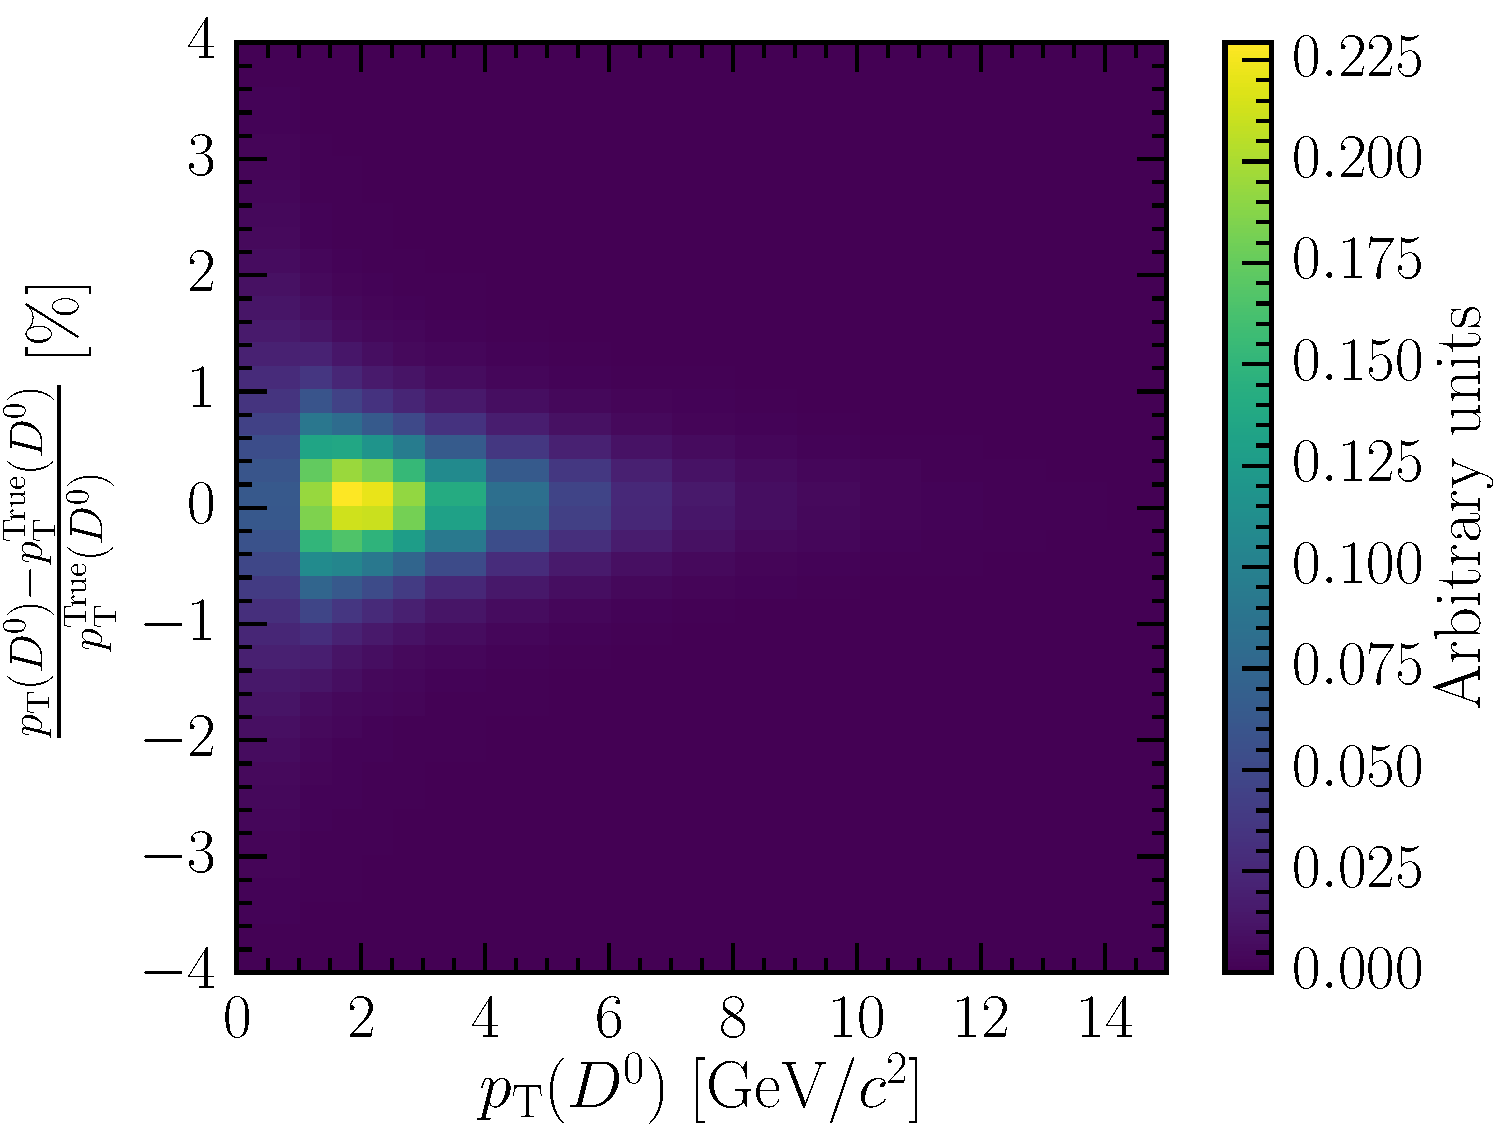
\includegraphics[width=\textwidth]{production/efficiencies/D0ToKpi_PT_resolution}
    \caption{}
    \label{fig:prod:effs:reco:unfolding:PT:resolution}
  \end{subfigure}
  \begin{subfigure}[b]{0.5\textwidth}
    \centering
    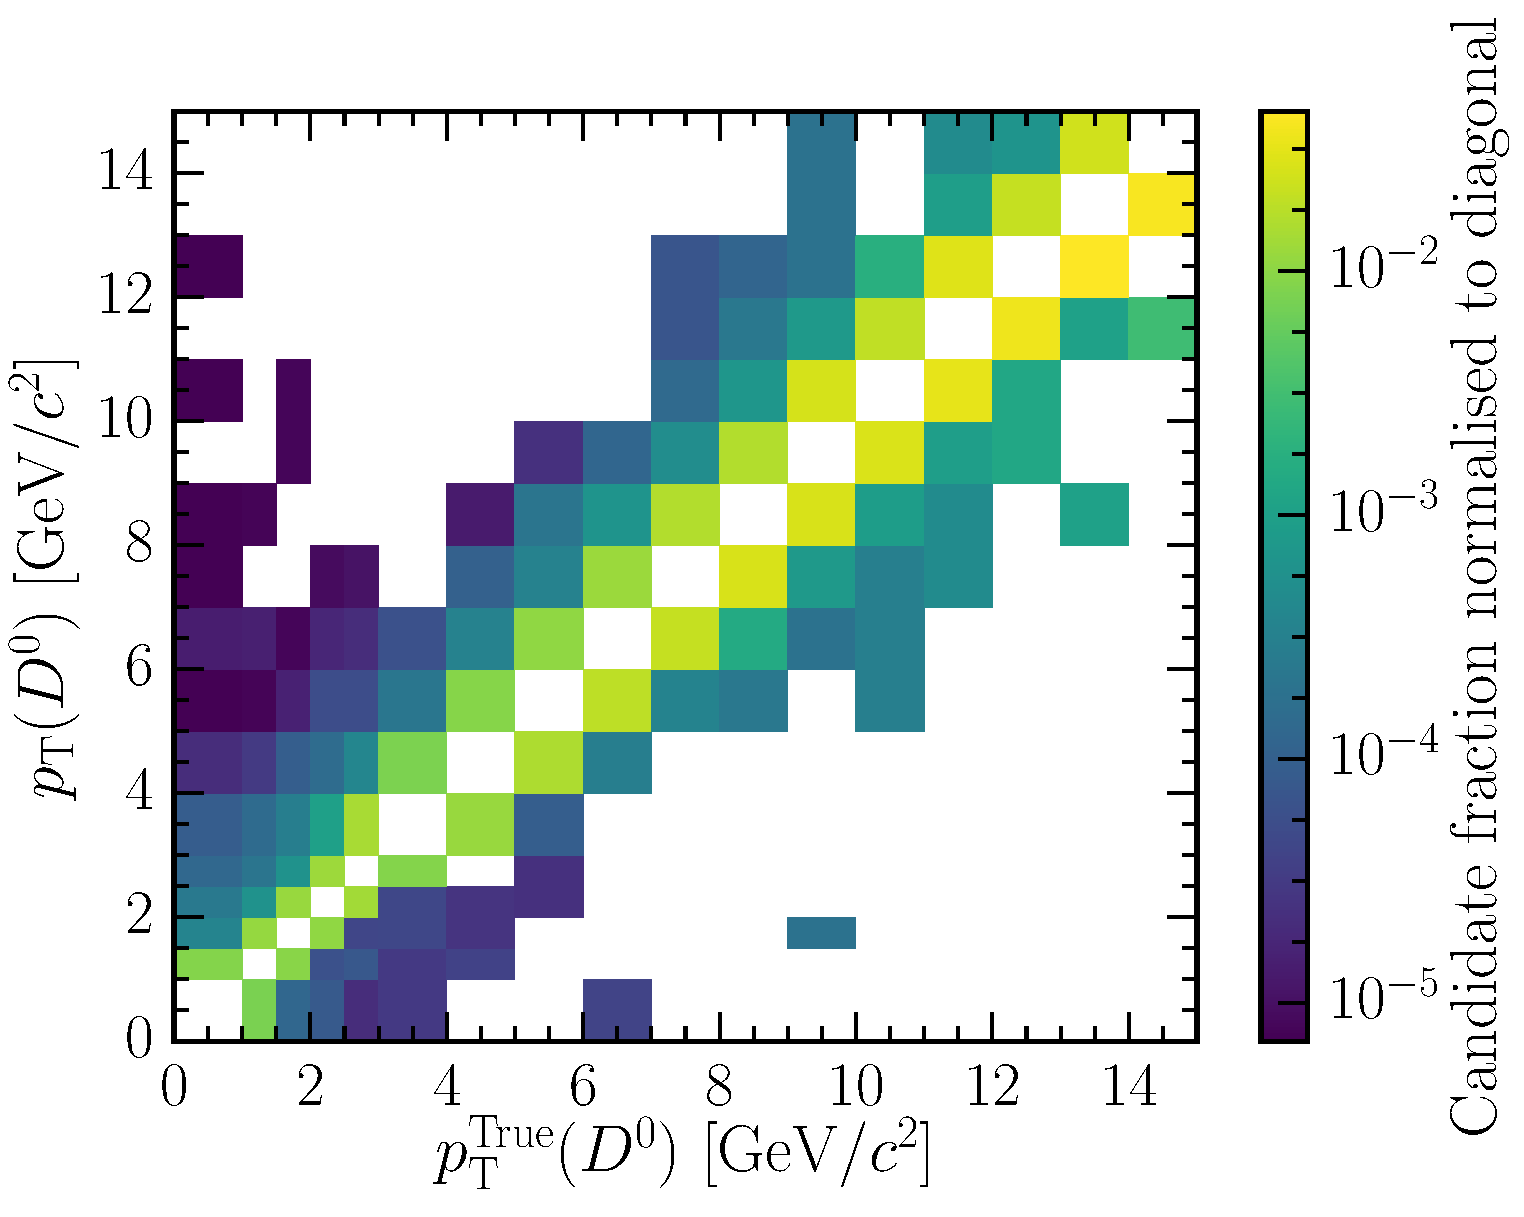
\includegraphics[width=\textwidth]{production/efficiencies/D0ToKpi_PT_migration_matrix}
    \caption{}
    \label{fig:prod:effs:reco:unfolding:PT:migration}
  \end{subfigure}
  \caption{%
    The difference between true and reconstructed \PDzero\ \pT\, normalised by 
    true \PDzero\ \pT, in bins of reconstructed 
    \pT~(\subref*{fig:prod:effs:reco:unfolding:PT:resolution}), and a migration 
    matrix~(\subref*{fig:prod:effs:reco:unfolding:PT:migration}) showing the 
    fraction of candidates that migrate within a true \pT\ bin, relative to the 
    diagonal (where there is no migration).
  }
  \label{fig:prod:effs:reco:unfolding:PT}
\end{figure}

\begin{figure}
  \begin{subfigure}[b]{0.5\textwidth}
    \centering
    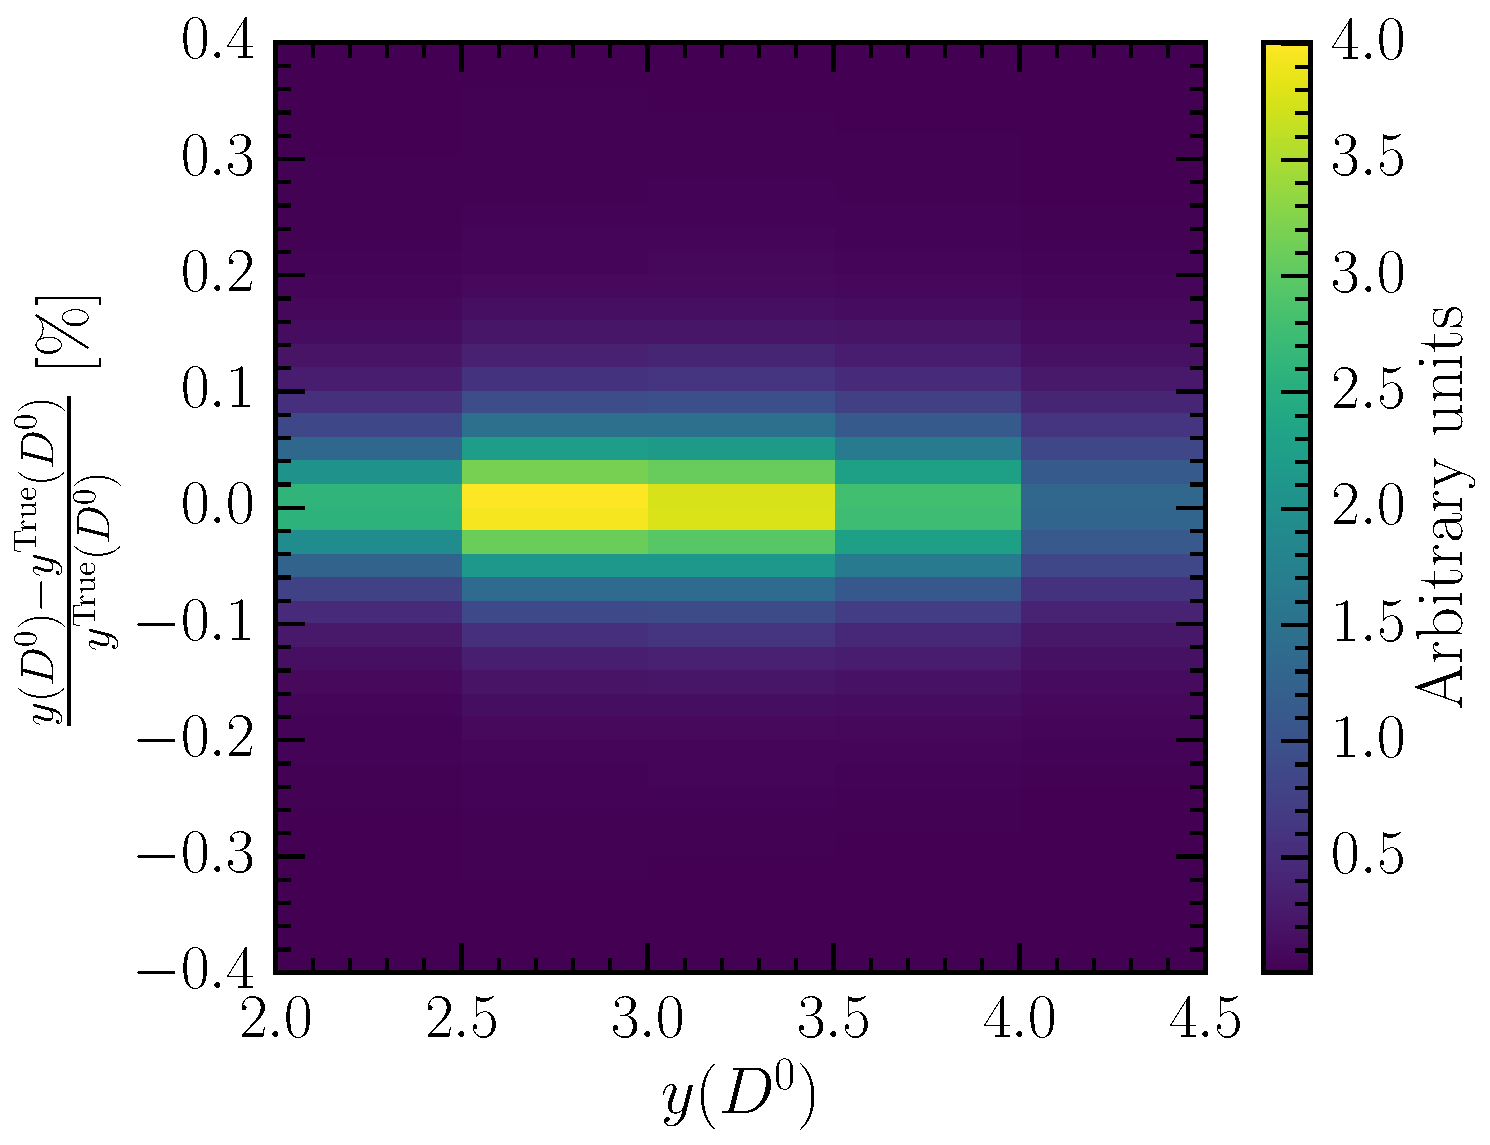
\includegraphics[width=\textwidth]{production/efficiencies/D0ToKpi_y_resolution}
    \caption{}
    \label{fig:prod:effs:reco:unfolding:y:resolution}
  \end{subfigure}
  \begin{subfigure}[b]{0.5\textwidth}
    \centering
    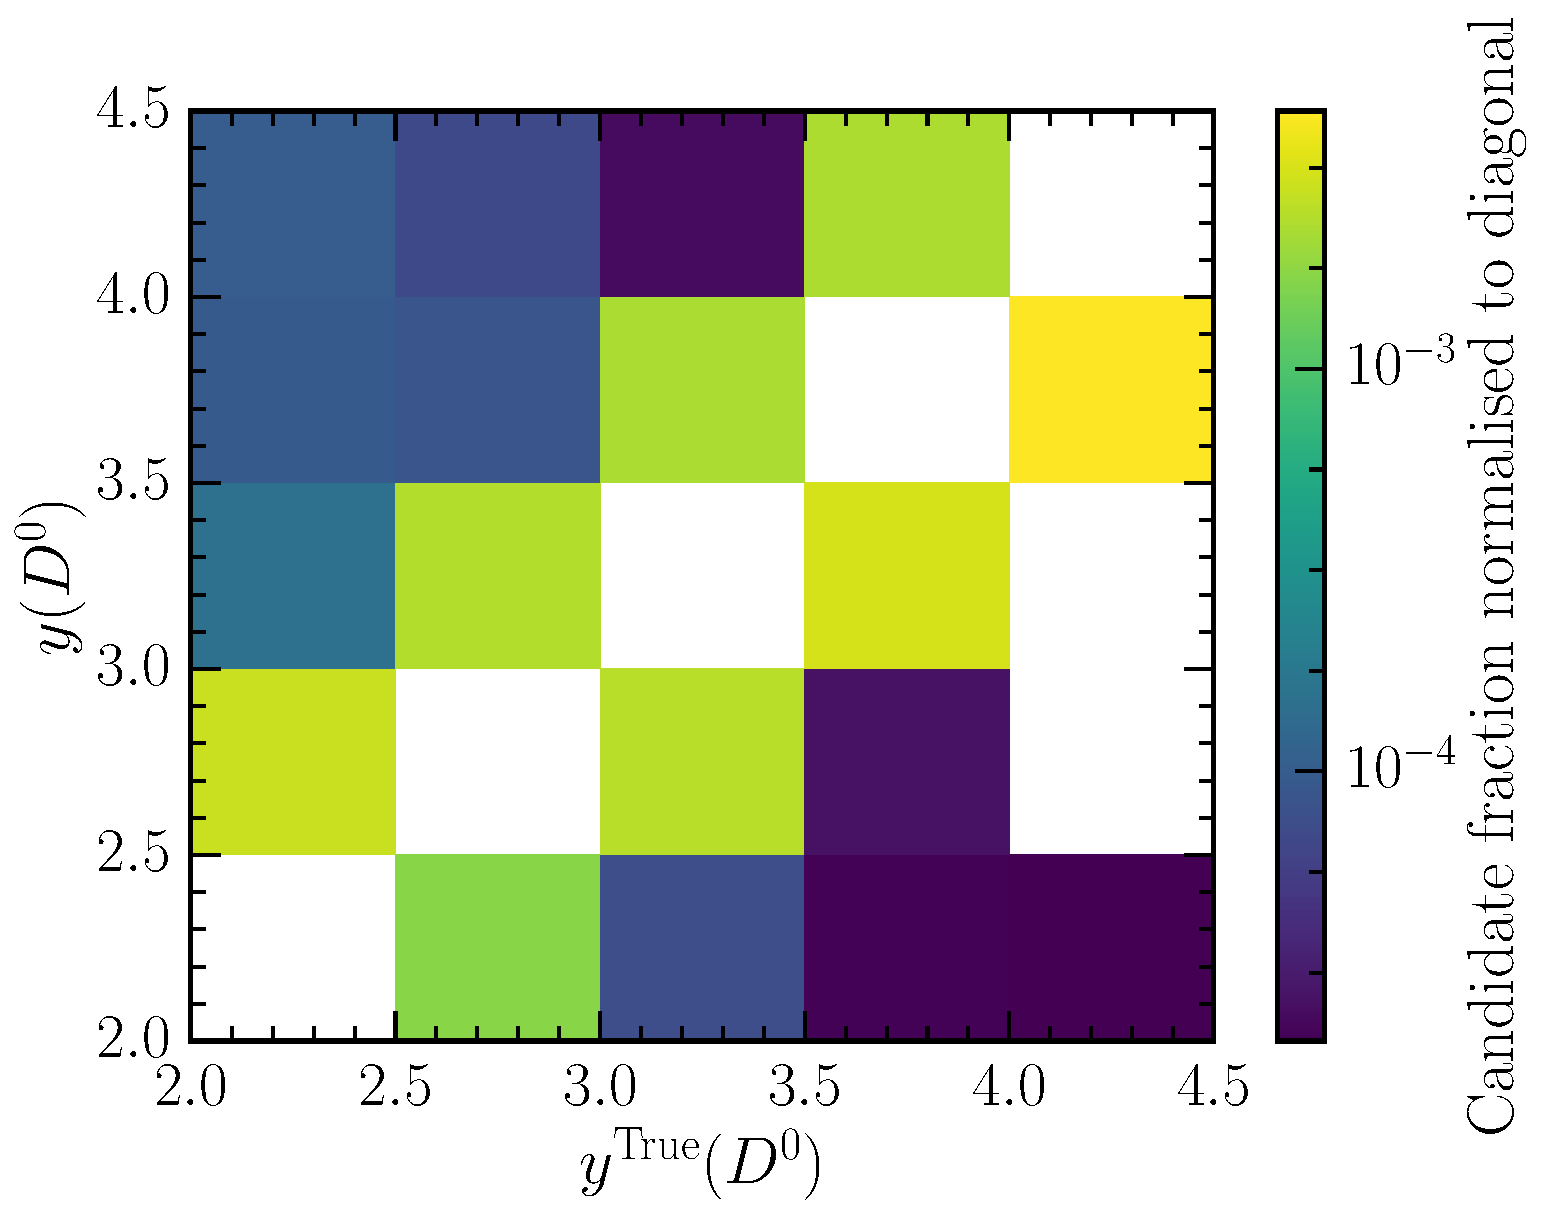
\includegraphics[width=\textwidth]{production/efficiencies/D0ToKpi_y_migration_matrix}
    \caption{}
    \label{fig:prod:effs:reco:unfolding:y:migration}
  \end{subfigure}
  \caption{%
    The difference between true and reconstructed \PDzero\ rapidity, normalised 
    by true \PDzero\ rapidity, in bins of reconstructed 
    rapidity~(\subref*{fig:prod:effs:reco:unfolding:y:resolution}), and a 
    migration matrix~(\subref*{fig:prod:effs:reco:unfolding:y:migration}) 
    showing the fraction of candidates that migrate within a true rapidity bin, 
    relative to the diagonal (where there is no migration).
  }
  \label{fig:prod:effs:reco:unfolding:y}
\end{figure}

\subsection{Truth matching inefficiency}
\label{chap:prod:effs:truth}

The evaluation of \cref{eqn:prod:effs:reco} requires that the reconstructed
objects, tracks and vertices, be correctly associated back to the `truth-level'
information, that is the \ac{MC} objects which were generated and then
propagated through the detector simulation.
The truth-matching procedure is described in \cref{chap:intro:lhcb:simulation}.
The background category information is used to filter the \ac{MC} such that the
number of remaining candidates are simply counted to obtain the input to some
efficiency computation, such as \cref{eqn:prod:effs:reco}.
However, the requirement that at least \SI{70}{\percent} of a track's hits are 
matched to hits created by a single \ac{MC} particle is not \SI{100}{\percent} 
efficient at accepting signal.
The magnitude of the size of the inefficiency can be determined by counting the
number of signal decays that fail the truth matching requirement.
\cref{fig:prod:effs:truth:categories} shows the \PDzero and \PDplus mass
distributions for the various background categories.
The `ghost' category exhibits a peak identical in nature to that seen in the
`signal' category.
As not all signal decays that are truly reconstructed will be counted as such
when only the `signal' category is considered, associated efficiencies are
underestimated.

Given that the number of correctly matched signal decays is $N$, and the number
of incorrectly labelled signal decays is $U$, the selection efficiency defined
in \cref{eqn:prod:effs:reco} is incorrect by a factor
\begin{equation}
  \efftruth = \frac{U+N}{N}.
  \label{eqn:prod:effs:truth}
\end{equation}
The number of decays passing the signal requirement is used for $N$, and $U$ is
measured with a maximum likelihood fit to the mass or \deltam\ distribution of
the decays not passing the requirement.
As shown in \cref{fig:prod:effs:truth:categories}, the fraction of incorrectly
identified signal decays is small, and so a single fit is performed with the
data integrated across all \pTy\ bins, and a single correction factor is
measured.
The details of the fit are identical to those for the mass fits used in the
charm yield extraction with real data, described in
\cref{chap:prod:fitting:mass}.
The result of the fits to the \DzToKpi\ and the \DpToKpipi\ simulation are
shown in \cref{fig:prod:effs:truth:fit}.
Table~\ref{tab:prod:effs:truth_matching} lists the correction factors obtained.

\begin{figure}
  \begin{subfigure}[b]{0.5\textwidth}
    \centering
    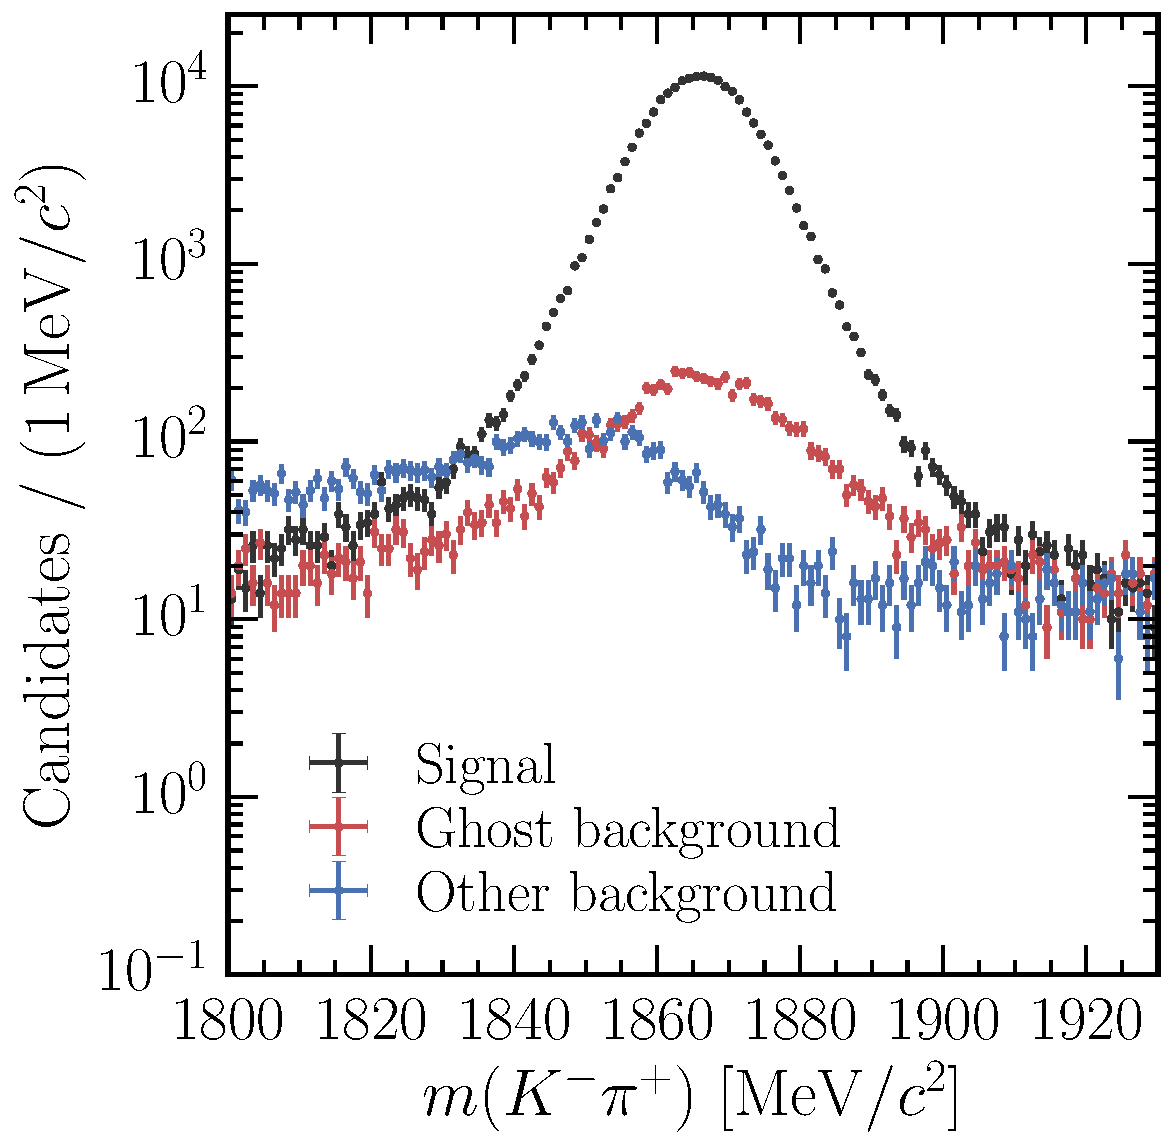
\includegraphics[width=\textwidth]{production/efficiencies/D0ToKpi_BKGCAT}
    \caption{\PDzero}
    \label{fig:prod:effs:truth:categories:D0ToKpi}
  \end{subfigure}
  \begin{subfigure}[b]{0.5\textwidth}
    \centering
    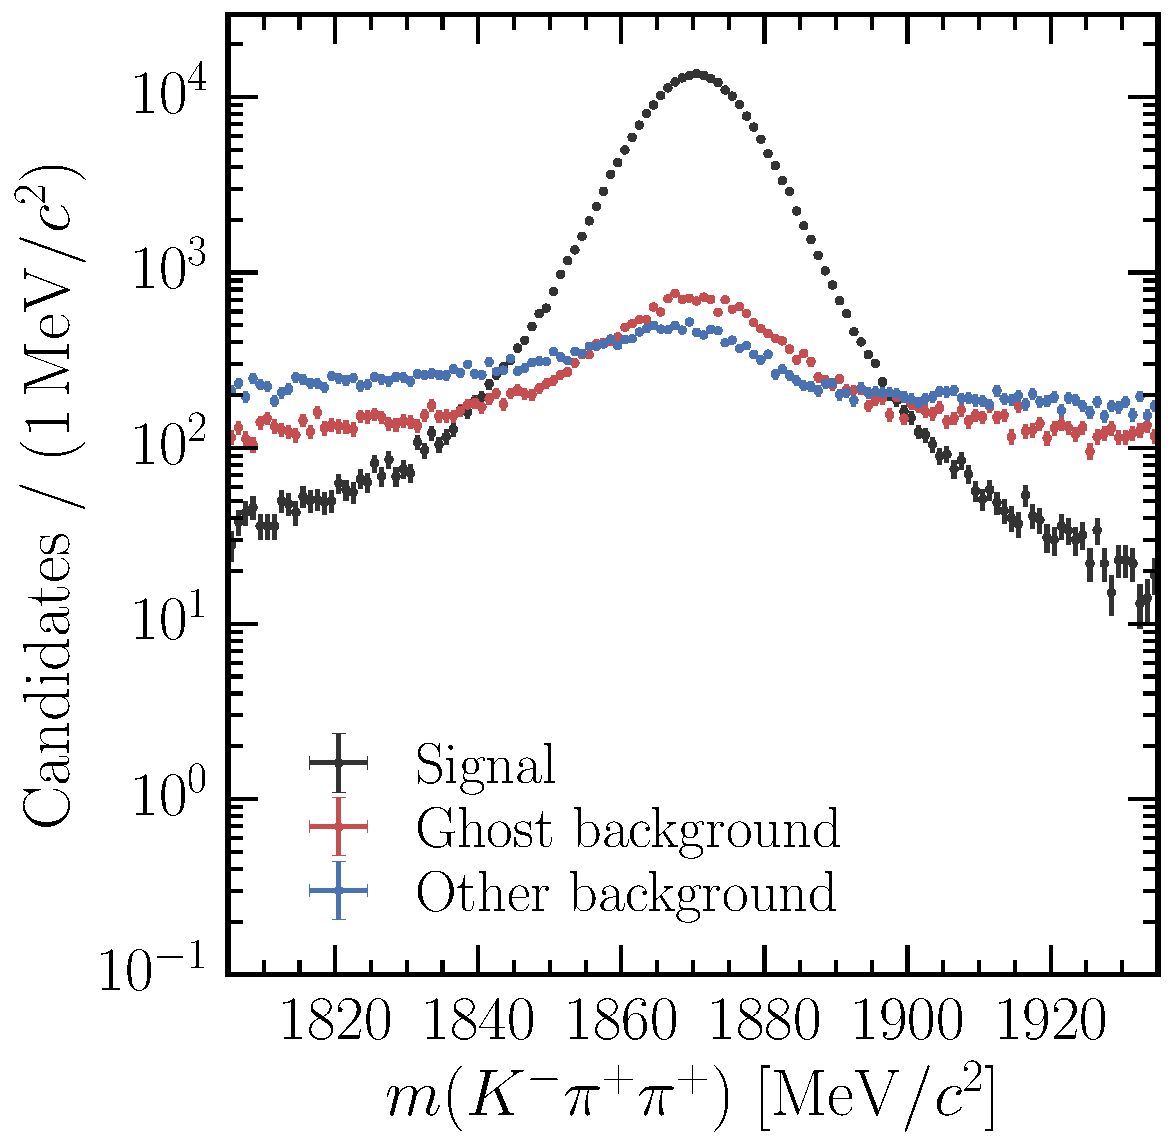
\includegraphics[width=\textwidth]{production/efficiencies/DpToKpipi_BKGCAT}
    \caption{\PDplus}
    \label{fig:prod:effs:truth:categories:DpToKpipi}
  \end{subfigure}
  \caption{%
    Mass distributions of \ac{MC}
    \PDzero~(\subref*{fig:prod:effs:truth:categories:D0ToKpi}) and
    \PDplus~(\subref*{fig:prod:effs:truth:categories:DpToKpipi}) candidates for
    various background categories, as indicated in the legends.
    The most prominent features are the signal-like peak in the `ghost'
    distribution, indicative of a truth-matching inefficiency, and the long
    tail extending below the mass peak in the `other' distribution, which
    mostly consists of partially reconstructed physics backgrounds such as
    \decay{\PDzero}{\PKminus\Ppiplus\Ppizero} and
    \decay{\PDplus}{\PKminus\Ppiplus\Ppiplus\Ppizero}.
  }
  \label{fig:prod:effs:truth:categories}
\end{figure}

\begin{figure}
  \begin{subfigure}[b]{0.5\textwidth}
    \centering
    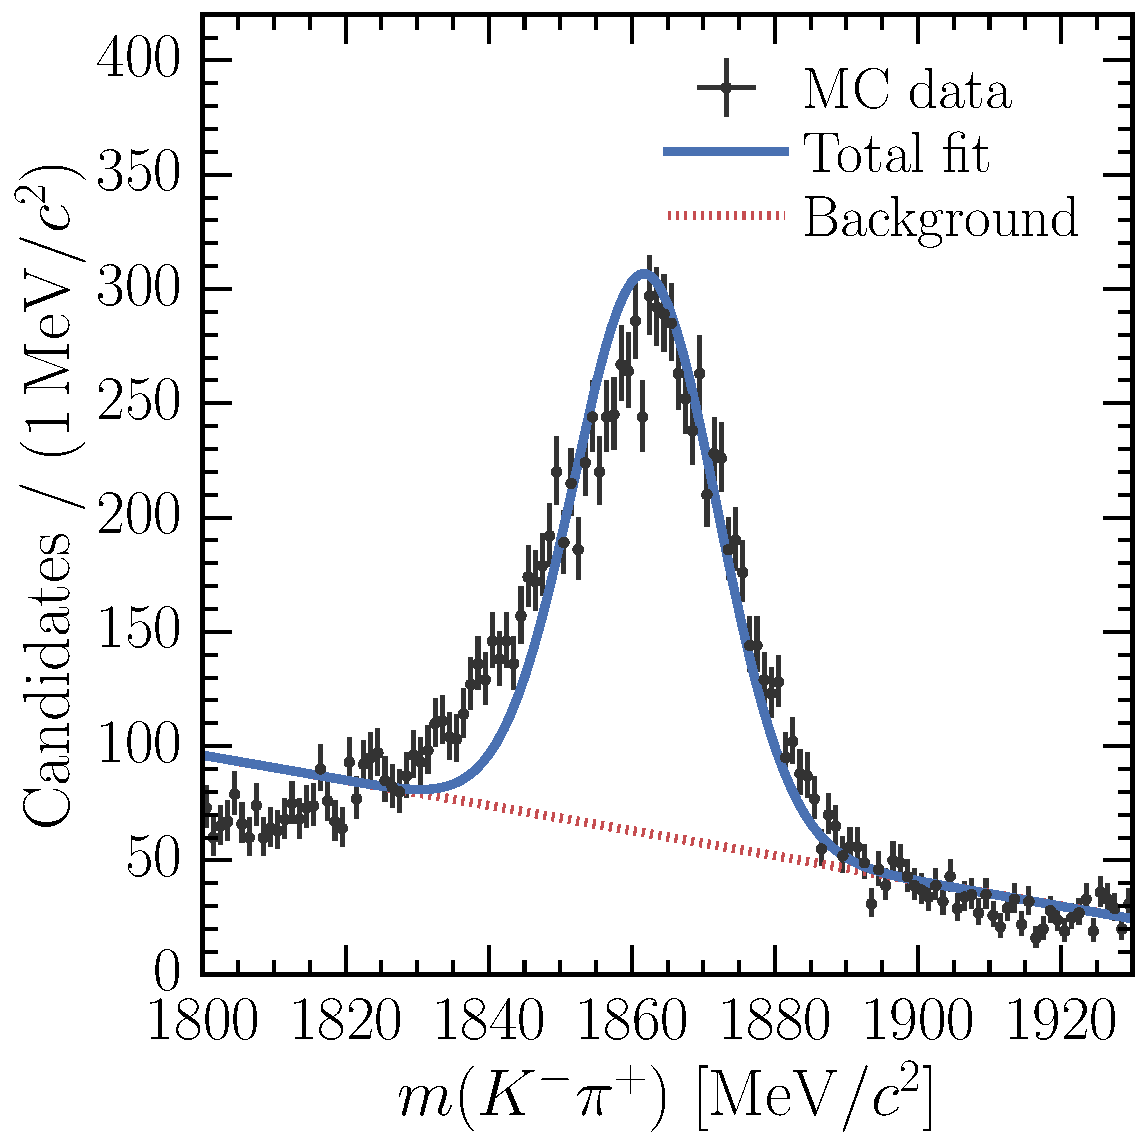
\includegraphics[width=\textwidth]{production/efficiencies/D0ToKpi_BKGCAT_fit}
    \caption{\DzToKpi}
    \label{fig:prod:effs:truth:fit:D0ToKpi}
  \end{subfigure}
  \begin{subfigure}[b]{0.5\textwidth}
    \centering
    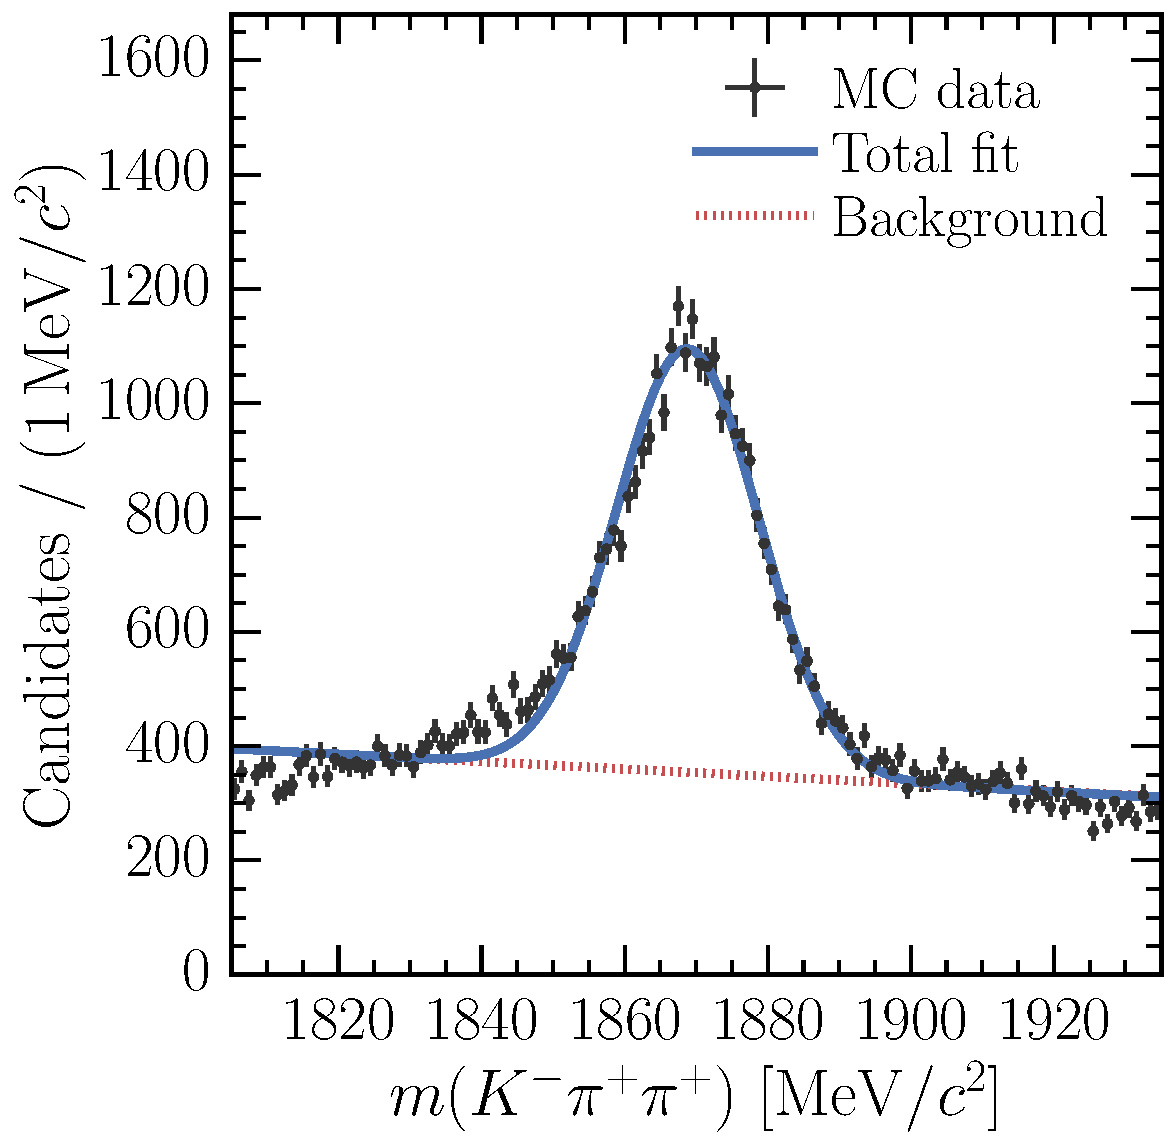
\includegraphics[width=\textwidth]{production/efficiencies/DpToKpipi_BKGCAT_fit}
    \caption{\DpToKpipi}
    \label{fig:prod:effs:truth:fit:DpToKpipi}
  \end{subfigure}
  \caption{%
    Mass distributions of \ac{MC}
    \PDzero~(\subref*{fig:prod:effs:truth:fit:D0ToKpi}) and
    \PDplus~(\subref*{fig:prod:effs:truth:fit:DpToKpipi}) candidates not
    passing the `signal' truth-matching requirement, that is the sum of the
    ``Ghost'' and ``Other'' categories shown in
    \cref{fig:prod:effs:truth:categories}.
    Overlaid on each distribution is the result of a maximum likelihood fit,
    with the total model shown as a blue curve, and the background model as a
    red dotted line.
  }
  \label{fig:prod:effs:truth:fit}
\end{figure}

\begin{table}
  \centering
  \caption{%
    Efficiency $1/\efftruth$ of
    the truth matching requirement applied in the simulation.
  }
  \label{tab:prod:effs:truth_matching}
  \begin{tabular}{lc}
  \toprule
  Mode                 & $1/\efftruth$ (\%) \\
  \midrule
  \DzToKpi             & $98.68 \pm 0.06$   \\
  \DpToKpipi           & $96.53 \pm 0.58$   \\
  \DspTophipi          & $98.53 \pm 0.13$   \\
  \DstToDzpi, \DzToKpi & $96.85 \pm 0.09$   \\
  \bottomrule
\end{tabular}

\end{table}

\subsection{Tracking efficiency correction}
\label{chap:prod:effs:tracking}

The tracking efficiency measures the efficiency for a charged particle to be
reconstructed as a track, and is part of the definition of the reconstruction
efficiency in \cref{eqn:prod:effs:reco}.
A data-driven technique is used to compute correction factors based on the
observed differences between the data and the \ac{MC}.

Only long tracks are used in this analysis, which requires that the particles
create hits in the \velo\ and in the T stations.
Hits in the \ttracker\ are not required to form long tracks, although matching
hits are added to tracks to improve their momentum resolution.
To measure the efficiency of long track creation, \JpsiTomumu\ decays are
reconstructed using a `tag-and-probe' technique, where one particle is fully
reconstructed as a long track and the other track is created using track
segments made only using information from the muon stations.
The momentum of the latter track, the `probe', can be inferred by treating the
magnetic field as an optical system that imparts a momentum `kick' in the $x$
direction.
By assuming the muon track segment was made by a particle originating from the
\ac{PV}, the probe segment can be extrapolated back from the muon stations to
the $yz$ plane where the kick is modelled, and then the difference in slopes
between the \ac{PV}-plane line and the probe track gives the probe momentum.
The invariant mass of the dimuon system can then be computed and the
distribution can be used to distinguish between backgrounds and true \PJpsi
decays.
The mass resolution of \JpsiTomumu\ decays reconstructed using long+muon tracks
is about \SI{200}{\MeVcc}, to be compared with a resolution of about
\SI{16}{\MeVcc} using long+long tracks.
To improve the mass resolution, the muon tracks are combined with hits in the
\ttracker, improving the resolution to around
\SI{57}{\MeVcc}~\cite{Aaij:2014pwa,DeCian:2013zua}.

The tracking efficiency is evaluated as the ratio of \PJpsi mesons
reconstructed using the long+muon+\ttracker\ method, with those that can
\emph{also} be reconstructed using the long+long method
\begin{equation}
  \eff_{\text{Tracking}} =
  \frac{%
    N_{\text{long+long}|\text{long+muon+TT}}
  }{%
    N_{\text{long+muon+TT}}
  }.
  \label{eqn:prod:effs:tracking_eff}
\end{equation}
A long track in an event is considered as `matched' to the probe track if there
is a \SI{70}{\percent} overlap of their hits in the muon stations.
The tag-and-probe method is performed using real data and \ac{MC}, and a ratio
is formed
\begin{equation}
  \efftracking = \frac{%
    \eff_{\text{Tracking}}^{\text{Data}}
  }{%
    \eff_{\text{Tracking}}^{\text{MC}}
  }.
  \label{eqn:prod:effs:tracking_ratio}
\end{equation}
This ratio is evaluated in bins of probe track momentum and
pseudorapidity, as the tracking efficiency is found to vary as a function
of these variables, and is shown in \cref{fig:prod:effs:tracking_table}.
As it is found to also vary as a function of the total number of reconstructed
long tracks in the event, the input tracks in the \ac{MC} are weighted such
that the event multiplicity distributions match those in the data.

The correction factor in \cref{eqn:prod:effs:tracking_ratio} can be applied to
the tracking efficiency found using any decay, as it is only a function of
\ptot\ and \Eta.
It is then applied to the reconstruction efficiency in
\cref{eqn:prod:effs:reco}, where for a single decay the total correction factor
is the product of the correction factors for all the tracks comprising the
final states.
Tracking efficiency correction factors for \DzToKpi\ and \DpToKpipi\ are given
in \cref{tab:prod:effs:tracking:dztokpi,tab:prod:effs:tracking:dptokpipi}.

The correction factors given do not account for the differences between muon
and hadron interactions with the detector.
These differences will result in different tracking efficiencies, which may not
be the same between data and \ac{MC}.
The effect of these differences will be discussed in the context of systematic
uncertainties in \cref{chap:prod:syst:tracking}.

\begin{figure}
  \centering
  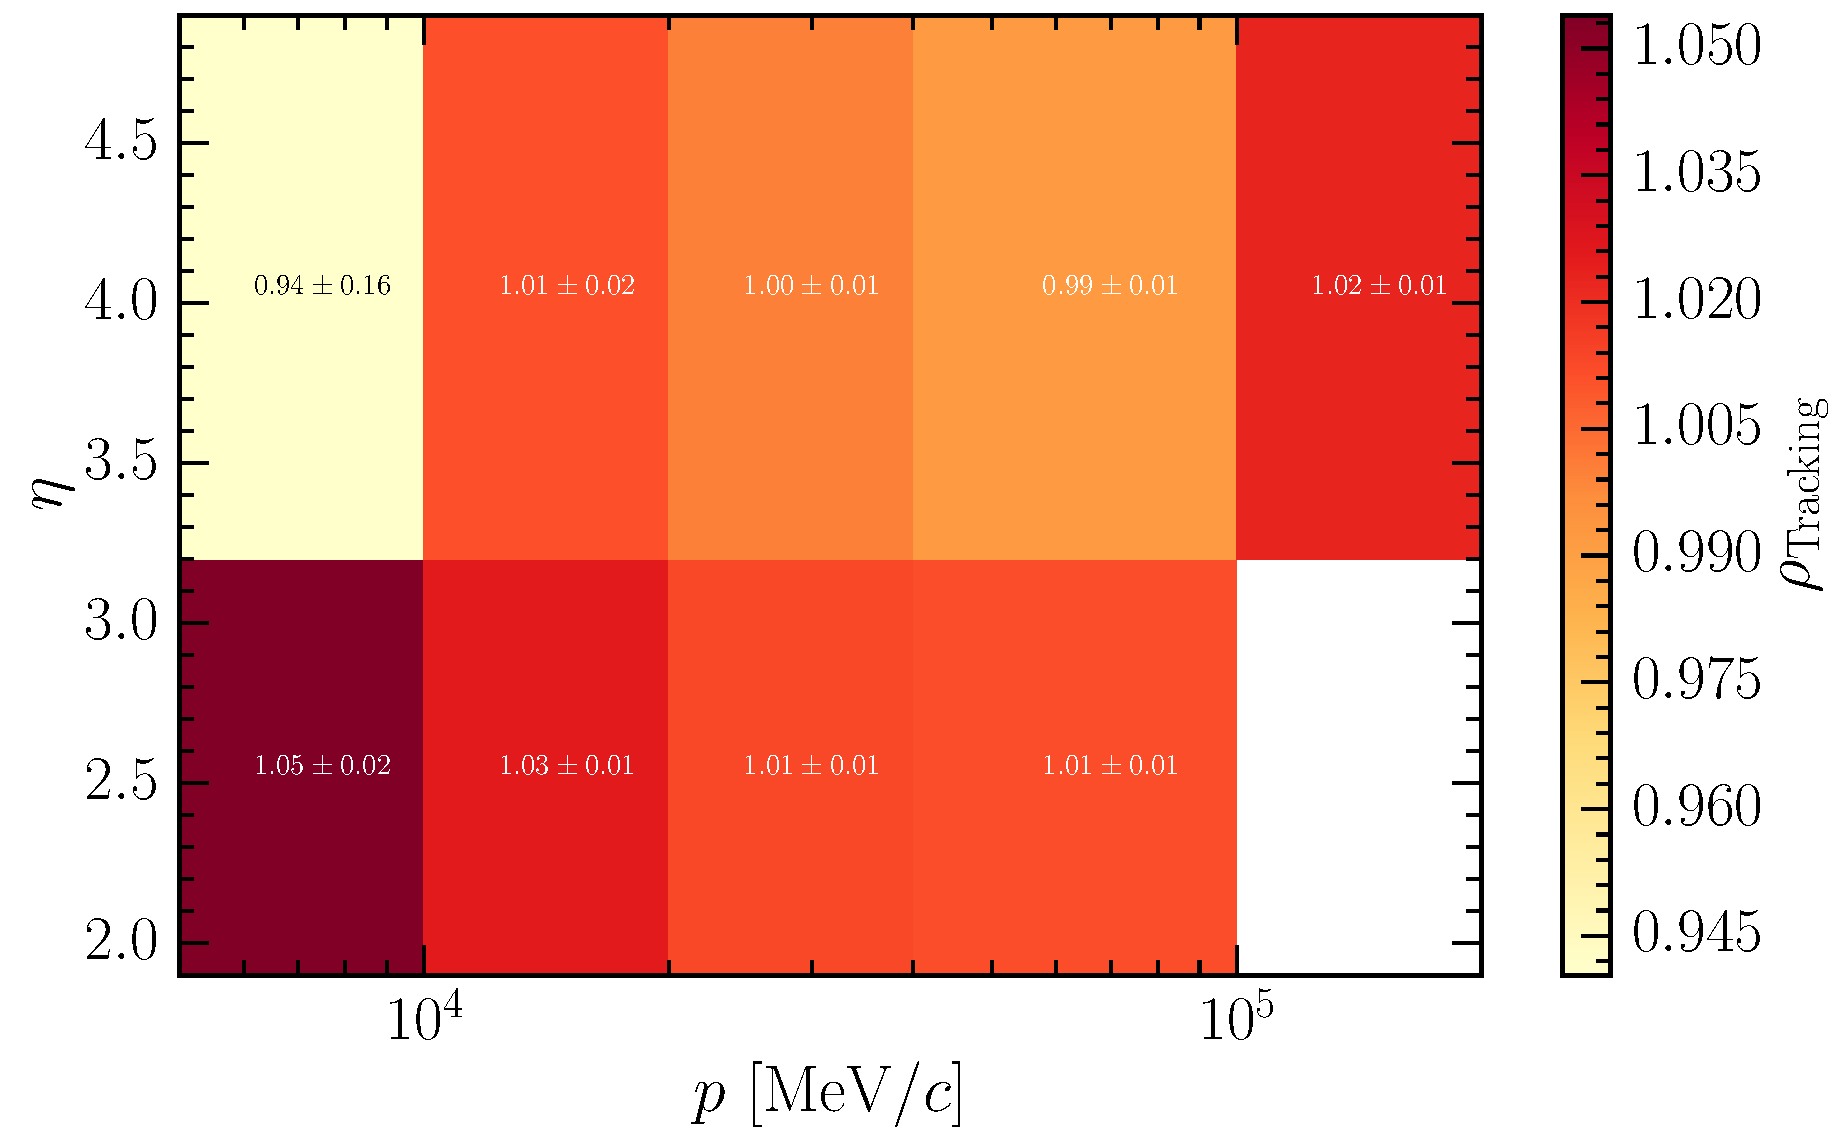
\includegraphics[width=\textwidth]{production/efficiencies/tracking_correction_table}
  \caption{%
    Tracking efficiency correction factors \efftracking\ in bins of track
    momentum and pseudorapidity.
    The value is labelled in each bin, along with the statistical uncertainty
    on those values due to the finite size of the calibration datasets.
    Bins in which a measurement could not be made are empty.
  }
  \label{fig:prod:effs:tracking_table}
\end{figure}

Combining the truth-matching efficiency and tracking efficiency correction
factors, the `corrected reconstruction' efficiency $\effreco'$ can be
considered to be
\begin{equation}
  \effreco' = \efftruth\times\efftracking\times\effreco.
  \label{eqn:prod:effs:reco_corrected}
\end{equation}

\section{Selection}
\label{chap:prod:effs:sel}

At this stage, the efficiency chain includes the effects of the detector
acceptance, the reconstruction, the truth-matching used to evaluate the
reconstruction efficiency, and the data-\ac{MC} differences in the tracking
efficiency.
What it left is the selection efficiencies due to the online and offline
selections, as described in \cref{chap:prod:sel}.
For simplicity, the `online' and `offline' selection are treated as a single
requirement, with the caveat that \ac{PID} requirements are not included.
The \ac{PID} efficiency can be computed using data-driven methods, and will be
described in \cref{chap:prod:effs:pid}.

The \lzero\ trigger selects bunch-bunch crossings randomly at a predetermined
rate, and so the \lzero\ efficiency is just the ratio of accepted crossings to
the total number, or equivalently
\begin{equation}
  \efflzero = \frac{%
    R_{\nobias}
  }{%
    \ncollbunches\revfreq
  },
  \label{eqn:prod:effs:sel:l0}
\end{equation}
where $R_{\nobias}$ is the rate at which the \lzero\ trigger was programmed to
accept crossings; \ncollbunches\ is the number of bunches in the \ac{LHC} which
collided at the \lhcb\ \acl{LHCIP}; and \revfreq\ is the bunch revolution
frequency of \SI{11.246}{\kilo\hertz}~\cite{Bruning:2004ej}.
Both $R_{\nobias}$ and \ncollbunches\ can vary as a function of the \ac{LHC}
fill, and hence so can $\eff_{\nobias}$.
The corresponding values are tabulated in
\cref{tab:prod:sel:online:l0_nobias_rateeff}.

The combined \hltone, \hlttwo, and offline selection efficiency is computed as
the ratio of the number of truth-matched decays passing the full selection (but
without \ac{PID} requirements) to the number of truth-matched, reconstructed
decays, giving
\begin{equation}
  \efftrig \times \effoffline = \effselection = \efflzero \times \frac{%
    N_{\text{Selected}|\text{Reconstructed}}
  }{%
    N_{\text{Reconstructed}}
  }.
  \label{eqn:prod:effs:sel}
\end{equation}
Selection efficiencies for \DzToKpi\ and \DpToKpipi\ are given in
\cref{tab:prod:effs:sel:dztokpi,tab:prod:effs:sel:dptokpipi}.

\section{Particle identification}
\label{chap:prod:effs:pid}

The \ac{PID} efficiency \effpid\ is the efficiency of a decay to pass all
requirements on the variables that are discriminatory between particle species.
The variables are those in the \acf{DLL} family, whose computation is described
in \cref{chap:intro:lhcb:detector:pid}.
This analysis uses the \dllkpi\ variable to discriminate between kaon and pion
tracks, with the exception of the soft pion in the \DstToDzpi\ decay on which
no \ac{PID} requirement is made.

It is assumed that the efficiency of a \ac{PID} cut for a given particle type
can be parameterised as a function of three variables: the track momentum
\ptot, the track pseudorapidity \Eta, and a measure of the detector occupancy.
These particular variables are chosen as the performance of the \rich\
detectors is known to depend them~\cite{Adinolfi:2012qfa}.
As a measure of the detector occupancy, the number \nspd\ of hits in the \spd\
detector is used.

A clean sample of \DzToKpi\ decays can be obtained without the use of \ac{PID}
information.
The \DzToKpi\ decay is reconstructed, and \PDzero mesons are then combined with
the remaining tracks in the event to form candidate \DstToDzpi\ decays.
Kaon (pion) candidates are those with the opposite (same) electric charge as
the pion from the \PDstarp.
Mis-identifications of other true \PDzero decays, such as
\decay{\PDzero}{\Ppiplus\Ppiminus} and \decay{\PDzero}{\PKplus\PKminus}, can be
resolved in the \PDzero invariant mass spectrum due to the high momentum
resolution of the detector, and true \PDstarp\ decays can be separated from
combinatorial background in the \deltam\ distribution.

The sample of \PDstarp-tagged \PDzero decays is referred to here as the
calibration sample, and has a \SI{20}{\percent} overlap with the sample used
for the cross-section measurement.
This is partly due to the different selection strategy that is necessary when
\ac{PID} information is ignored, and also due to inclusive trigger requirements
imposed on the calibration sample.
To compute the efficiency of a given \ac{PID} requirement on either a kaon or a
pion track, kaons or pions from the calibration sample are partitioned in
\ptot, \Eta, and \nspd\ as a three-dimensional histogram.
The number $C_{i}$ of signal tracks in the $i$th bin is computed, and then the
number $C_{i}'$  of signal tracks after the \ac{PID} requirement is computed,
such that the efficiency in the $i$th bin is
\begin{equation}
  \eff_{i} = \frac{C_{i}'}{C_{i}}.
\end{equation}
It is assumed that the \ptotetanspd\ partitions are sufficiently small that the
\ac{PID} efficiency within a bin is single-valued.
The three-dimensional histogram of efficiencies is an estimate of the
efficiency model for the given \ac{PID} requirement on the given particle.

The track counts $C_{i}$ and $C_{i}'$ are obtained with a single
two-dimensional fit to the \PDzero mass and the \deltam\ distributions.
Weights are computed that can be used to statistically remove the background
contribution in variable distributions that are uncorrelated with the invariant
mass~\cite{Pivk:2004ty}.
As \ptot, \Eta, and \nspd\ are found to be uncorrelated with the fit variables,
these weights are used to compute $C_{i}$ by summing the weights of the tracks
that fall in the $i$th bin.
The weights are also used to compute $C_{i}'$ in the same way, as the \dll\
variables are found to be uncorrelated with the fit variables.
Once the efficiency in each \ptotetanspd\ bin is known, the \ac{PID}\
efficiency for the same cut on \emph{any} track can be evaluated by looking up
which bin the track falls into, and assigning the corresponding efficiency.

For the calibration sample, the average efficiency across the parameterisation
space can be expressed as
\begin{equation}
  \effpid = \frac{%
    \displaystyle\sum_{i \in \textnormal{bins}} C_{i}\eff_{i}
    }{%
    \displaystyle\sum_{i \in \textnormal{bins}} C_{i}
    }.
\end{equation}
For some other sample of tracks, referred to here as the reference
sample,\footnotemark\ the contents of each bin can be scaled by a weight
$w_{i}$ based on the fraction of the total reference sample size in the $i$th
bin relative to that of the calibration sample
\begin{equation}
  w_{i} = \frac{%
    R_{i}
  }{%
    C_{i}
  }\frac{%
    C
  }{%
    R
  },
  \label{eqn:prod:effs:pid:ref_weight}
\end{equation}
where $C_{i}$ ($R_{i}$) is the number of signal calibration (reference) tracks
in the $i$th bin, as before, and $C$ ($R$) is the total number of signal
calibration (reference) tracks in the sample.
The average \ac{PID} efficiency for the weighted reference sample is then
\begin{equation}
  \effpid = \frac{%
    \displaystyle\sum_{i \in \textnormal{bins}} w_{i}C_{i}\eff_{i}
  }{%
    \displaystyle\sum_{i \in \textnormal{bins}} w_{i}C_{i}
  }.
  \label{eqn:prod:effs:pid:single_track_ref_eff}
\end{equation}

\footnotetext{%
  It is the ``reference'' sample because it does not have to be equal to the
  sample of tracks in data one wishes to know the efficiencies for.
  It can be a sample of simulated data that describes the kinematics of the
  decay well, or even a different decay mode with similar properties (often
  called a control channel or a reference channel).
}

For this cross-section analysis, all the final states have multiple charged
tracks, of different species, upon which \ac{PID} requirements are made.
\Cref{eqn:prod:effs:pid:single_track_ref_eff} gives the average \ac{PID}
efficiency for a final state where a \ac{PID} requirement is made only on one
track, and so the formalism must be extended to the multi-track case.
The average efficiency is first modified by substituting
\cref{eqn:prod:effs:pid:ref_weight} into
\cref{eqn:prod:effs:pid:single_track_ref_eff} to give
\begin{equation}
  \effpid = \frac{%
    \displaystyle\sum_{i \in \textnormal{bins}} R_{i}\eff_{i}
  }{%
    \displaystyle\sum_{i \in \textnormal{bins}} R_{i}
  }
  = \frac{1}{R}\sum_{i \in \textnormal{bins}} R_{i}\eff_{i},
\end{equation}
and then expanding in terms of $a_{ij}$, the \emph{weight} of the $j$th
reference track in the $i$th \ptotetanspd\ bin
\begin{equation}
  \effpid = \frac{1}{R}
            \sum_{i \in \textnormal{bins}}\sum_{j} a_{ij}\eff_{i}.
  \label{eqn:prod:effs:pid:expanded_ref_eff}
\end{equation}
The weight term can account for the possibility of an impure reference sample,
where, for example, it can be the same type of background-subtracting weight as
used for the creation the efficiency histogram from the calibration sample.
With this, the \ac{PID} efficiency calculation can be thought of as either of
two equivalent methods: weighting the calibration sample to look like the
reference sample, as in \cref{eqn:prod:effs:pid:single_track_ref_eff}, or
assigning per-track efficiencies to the reference sample based on \ptotetanspd\
bins they fall into, as in \cref{eqn:prod:effs:pid:expanded_ref_eff}.
The latter can be generalised to multi-track efficiencies by summing over all
\emph{decays} in the reference sample, replacing the per-track efficiency by a
per-decay efficiency \effpiddecay
\begin{equation}
  \effpid = \frac{1}{R}\sum_{d\in\text{decays}} a_{d}\effpiddecay,
\end{equation}
where $a_{d}$ is the weight of the decay, and \effpiddecay\ is the \ac{PID}
efficiency for that decay.
The per-decay efficiency \effpiddecay\ for the case in which a \ac{PID}
requirement is made on only a single track is \effpidtrack, whilst for a
multi-track decay it is
\begin{equation}
  \effpiddecay = \prod_{t \in \textnormal{tracks}} \effpidtrack.
\end{equation}

In this analysis, the reference sample used for the calibration is the fully
selected data, which includes \ac{PID} cuts applied both in the trigger and
offline.
The use of a reference sample that includes \ac{PID} cuts is a valid approach
under the assumption that no efficiency bins have a reference sample size of
zero~\cite{Anderlini:2202412}.
The benefit is that one does not rely on a proxy or \ac{MC} dataset correctly
modelling the track kinematics, and the inter-track correlations.

The statistical component of the uncertainty on the \ac{PID} efficiency due to
the finite size of the calibration sample is computed via a series of
pseudo-experiments, which will be described in \cref{chap:prod:syst:pid:stat}.
As the reference sample is also of a finite size, there is an additional,
associated uncertainty on the per-decay \ac{PID} efficiency.
However, the reference sample is identical to the sample entering the fits
described in \cref{chap:prod:fitting}, and so this uncertainty is already
accounted for in the uncertainty on the fitted signal yields.

\subsection{Optimisation of \texorpdfstring{\ptotetanspd}{(p, eta, Nspd)} binning scheme}
\label{chap:prod:effs:pid:binning}

An assumption in the method of \ac{PID} calibration previously described is
that the \ac{PID} efficiency within a \ptotetanspd\ bin is single-valued.
This can be guaranteed by employing an infinitely fine binning.
In reality, this cannot be used due to the finite size of the calibration
sample.

\Cref{fig:prod:effs:pid:binning:kaon_no_optimisation} illustrates the
dependence of the efficiency of the kaon \ac{PID} requirement on kaon momentum,
as computed in equal-probability bins based on the calibration sample
populations.
The efficiency varies strongly with track momentum, and the equal-probability
binning can lead to neighbouring bins where the efficiency is near-constant, as
in the 14--\SI{25}{\GeVc} region where a single bin may be a sufficient model.
In addition, the relative softness of the reference sample distribution
(black), compared to that of the calibration sample (red), leads to a large
fraction of the reference data being covered by a single bin ($p <
\SI{14}{\GeVc}$).
If the efficiency varies strongly within the first bin, the average value of
the \ac{PID} efficiency in that bin is different for the reference and
calibration samples, and so estimating the reference efficiency with that
obtained from the calibration samples will give a biased result.

In an attempt to minimise potential biases in the evaluation of the \ac{PID}
efficiency on the reference sample, for each one-dimensional projection of the
\ptotetanspd\ distribution the following iterative procedure is used, assuming
each projection is initially partitioned as a single bin:
\begin{enumerate}
  \item Divide each bin into ten equal-probability sub-bins.
  \item For each bin:
    \begin{enumerate}
      \item Compute the \ac{PID} efficiency using the calibration sample in the
        bin \eff\ and in the ten sub-bins $\eff_{i}$, and evaluate a \chisq\
        statistic as
        \begin{equation}
          \chisq = \sum_{i}^{10} \frac{{(\eff - \eff_{i})}^{2}}{\unc{\eff_{i}}^{2}},
          \label{eqn:prod:effs:pid:bin_chisq}
        \end{equation}
      \item Compute the $p$-value of the \chisq\ value given 9 degrees of
        freedom. If $p < 0.001$, the null hypothesis that the \ac{PID}
        efficiency within the bin is constant is rejected, and so the bin
        should be divided in two. Otherwise, the bin is not split.
    \end{enumerate}
  \item For each bin that should be divided in two:
    \begin{enumerate}
      \item Divide the bin into twenty equal probability sub-bins.
      \item For each of the 19 new boundaries, compute the \chisq\ statistic in
        the union of the sub-bins below the boundary and in the union of the
        sub-bins above the boundary using \cref{eqn:prod:effs:pid:bin_chisq},
        and record the sum of the two \chisq\ values. The \chisq\ computation 
        made under the hypothesis that the efficiency within each union is 
        constant.
      \item Record the boundary with the smallest \chisq\ sum.
      \item If the two sub-bin unions either side of the recorded boundary do
        not each contain at least 2000 tracks, the original bin is not split.
        Otherwise, the original bin is split in two at the recorded boundary.
    \end{enumerate}
  \item If no additional bins were created in this iteration, stop.  Otherwise,
    repeat from Step 1
\end{enumerate}
The iteration stops when either all bins satisfy the $p$-value requirement or
no further divisions are possible due to the lower sample size limit.
The sample size limit of 2000 tracks was chosen to reduce the possibility that
the three one-dimensional binning schemes could be combined to form a
three-dimensional binning which contained empty bins.
\Cref{fig:prod:pid:binning:kaon,fig:prod:pid:binning:pion} shows the resulting
\ptotetanspd\ binning (dark red) for kaon and pion tracks.
It can be seen that there are still bins where the finer binning (blue) shows a
large variation in the efficiency.
The effect of this on the cross-section measurement is considered as a
systematic uncertainty in \cref{chap:prod:syst:pid}.

The \acl{PID} efficiencies computed using the calibration procedure are given
in \cref{tab:prod:effs:pid:dztokpi,tab:prod:effs:pid:dptokpipi} for \DzToKpi\
and \DpToKpipi.
The uncertainties given are those due to the finite size of the calibration
sample.

\begin{figure}
  \centering
  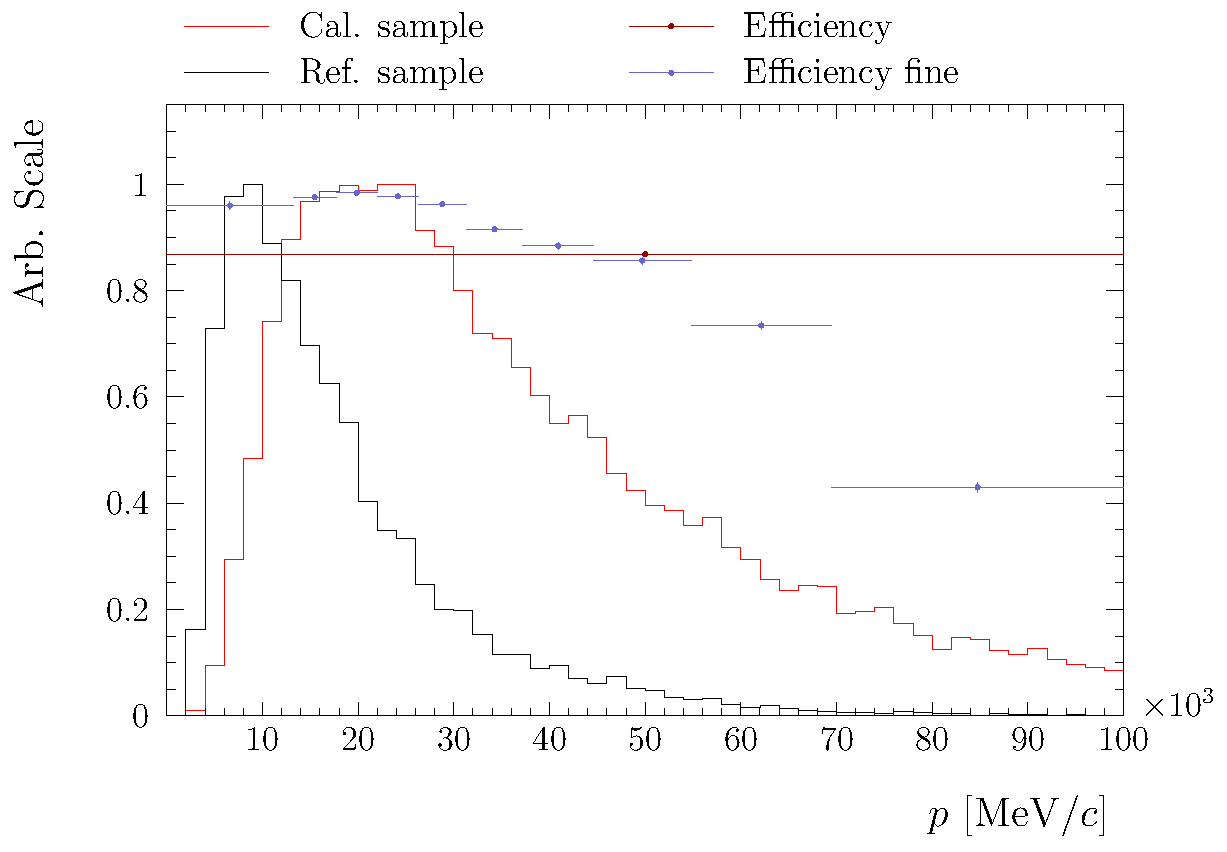
\includegraphics[width=\textwidth,trim={0 0 0 1.75cm},clip]{production/efficiencies/PID_binning_kaon_p_no_optimisation}
  \caption{%
    Unoptimised binning scheme (blue) for computing kaon \ac{PID} efficiencies.
    The kaon momentum distributions are shown for the calibration sample
    distribution (red) and the reference sample distribution (black).
  }
  \label{fig:prod:effs:pid:binning:kaon_no_optimisation}
\end{figure}

\section{Signal window}
\label{chap:prod:effs:signal_window}

As described in Section~\ref{chap:prod:fitting}, the number of prompt signal
candidates is measured by fitting the \lnipchisq\ distribution of candidates in
a signal window defined in the mass distribution.
This mass window requirement removes some signal candidates.
The efficiency of the requirement is evaluated by computing the fractional
integral of the signal component of the model $f_{\text{Sig.}}(m)$ fitted to
the mass distribution.
In the case of the \PDstarp measurement, there is an additional requirement
that the candidates used in the \lnipchisq\ fit fall in a signal window defined
in the \deltam\ distribution.
The efficiency of the \deltam\ signal window requirement is computed in the
same way as for the mass signal window requirement, except the signal component
of the model fitted to the \deltam\ distribution $g_{\text{Sig}}(\deltam)$ is
used.

To assign an uncertainty to the integrals, the fractional integral is
recomputed in a series of 500 pseudo-experiments.
Within each one, each shape parameter is assigned a value sampled from a
normal distribution with a mean as the `nominal' value of that parameter, the
value found by the fit, and with a width equal to the uncertainty on that
nominal value. Correlations between the different shape parameters are taken
into account by sampling parameter values from the covariance matrix found in
the nominal fit.
The variance on the deviation of the integrals, with respect to the integral
computed using the nominal shape parameter values, is taken as the square of
the uncertainty on the nominal integral value.

As the shape of some mass signal models are \pTy\ bin dependent, as described
in Section~\ref{chap:prod:fitting:details}, the signal window efficiency is computed
separately in each \pTy\ bin.
\Cref{tab:prod:effs:sigwin:dztokpi,tab:prod:effs:sigwin:dptokpipi}
give the per-bin signal window efficiencies for each mode.

\section{Uncertainties on efficiencies}
\label{chap:prod:effs:tot}

For the efficiencies computed by counting the number $N$ of decays before and
the number $k$ after some selection, the estimator \effest\ of the true
efficiency is taken to be $k/N$.
The application of the selection on the $N$ decays is considered as a binomial
process, with the probability $P$ to observe $k$ counts given the true
efficiency \eff\ and the number of initial $N$ counts given by
\begin{equation}
  P(k | \eff, N) = \begin{pmatrix}N\\k\end{pmatrix}\eff^{k}{(1 - \eff)}^{N - k}.
  \label{eqn:prod:effs:binomial_pdf}
\end{equation}
To utilise the \ac{MC} error propagation discussed in
\cref{chap:prod:introduction:uncertainties}, a \ac{PDF} of $\eff$ given $k$ and
$N$ is needed.
This can be found by using Bayes' theorem
\begin{equation}
  P(\eff | k, N) \propto P(k | \eff, N)P(\eff |N).
  \label{eqn:prod:effs:binomial_bayes}
\end{equation}
where $P(\eff | N)$ is the prior probability and $P(\eff | k, N)$ is the
posterior probability.
For this analysis, a flat prior in $\eff$ is chosen, encoding the belief that,
given only $N$, any value of \eff\ between 0 and 1 is reasonable.
Substituting such a prior and \cref{eqn:prod:effs:binomial_pdf} into
\cref{eqn:prod:effs:binomial_bayes}, the posterior becomes
\begin{equation}
  P(\eff | k, N) \propto \eff^{k}{(1 - \eff)}^{N - k}.
\end{equation}
This is the beta distribution $B(\alpha, \beta)$ for $\alpha = k + 1$ and
$\beta = N - k - 1$, and is what is used as the generating \ac{PDF} in the
\ac{MC} error propagation.

For the purposes of visualisation, it is useful to quote an uncertainty on the
estimator \effest.
The standard treatments of uncertainty evaluation on an efficiency can yield
symmetric uncertainties of zero, or even $\pm1\sigma$ intervals that include
unphysical efficiencies, when extreme values of $k$ and $N$ are
used~\cite{Paterno:2004cb}.
Instead, asymmetric \SI{68.2}{\percent} confidence intervals are computed using
the Agresti-Coull method~\cite{Agresti:2685469}, and are given as uncertainties
on all efficiencies computed as ratios of counts.

\begin{figure}
  \centering
  \begin{subfigure}[b]{0.7\textwidth}
    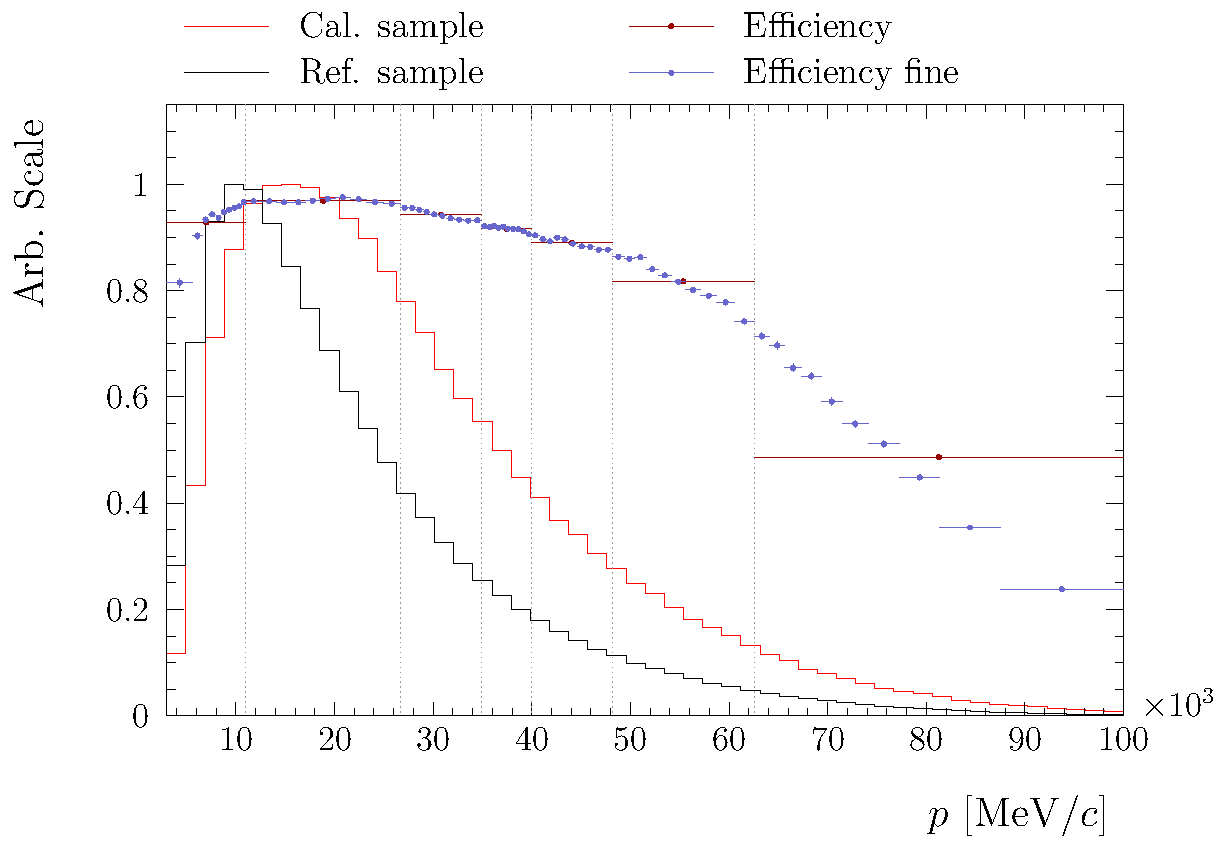
\includegraphics[width=\textwidth,trim={0 0 0 1.75cm},clip]{production/efficiencies/PID_binning_kaon_p}
    \caption{Track \ptot}
    \label{fig:prod:effs:pid:binning:kaon:p}
  \end{subfigure}
  \begin{subfigure}[b]{0.7\textwidth}
    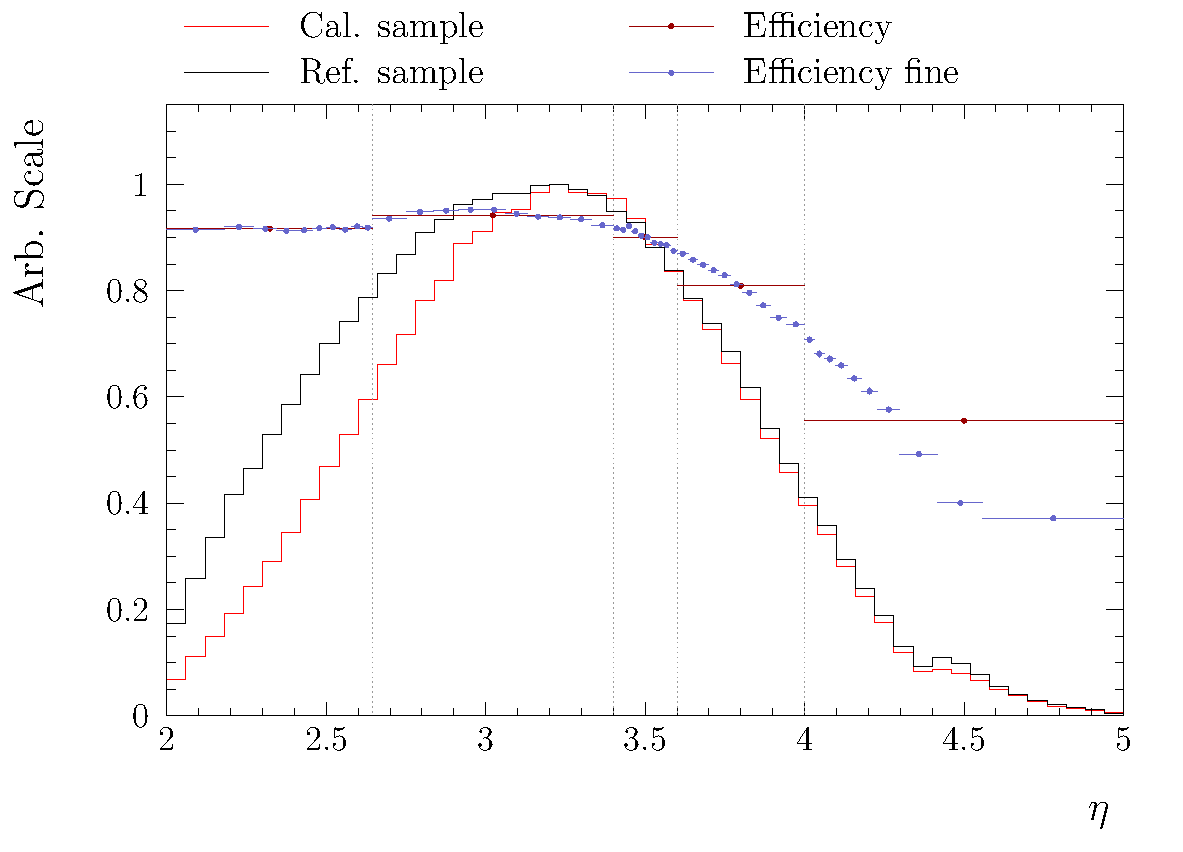
\includegraphics[width=\textwidth,trim={0 0 0 1.75cm},clip]{production/efficiencies/PID_binning_kaon_eta}
    \caption{Track \Eta}
    \label{fig:prod:effs:pid:binning:kaon:eta}
  \end{subfigure}
  % Increase spacing between rows so labels aren't too close to lower figures
  % \\[0.5cm]
  \begin{subfigure}[b]{0.7\textwidth}
    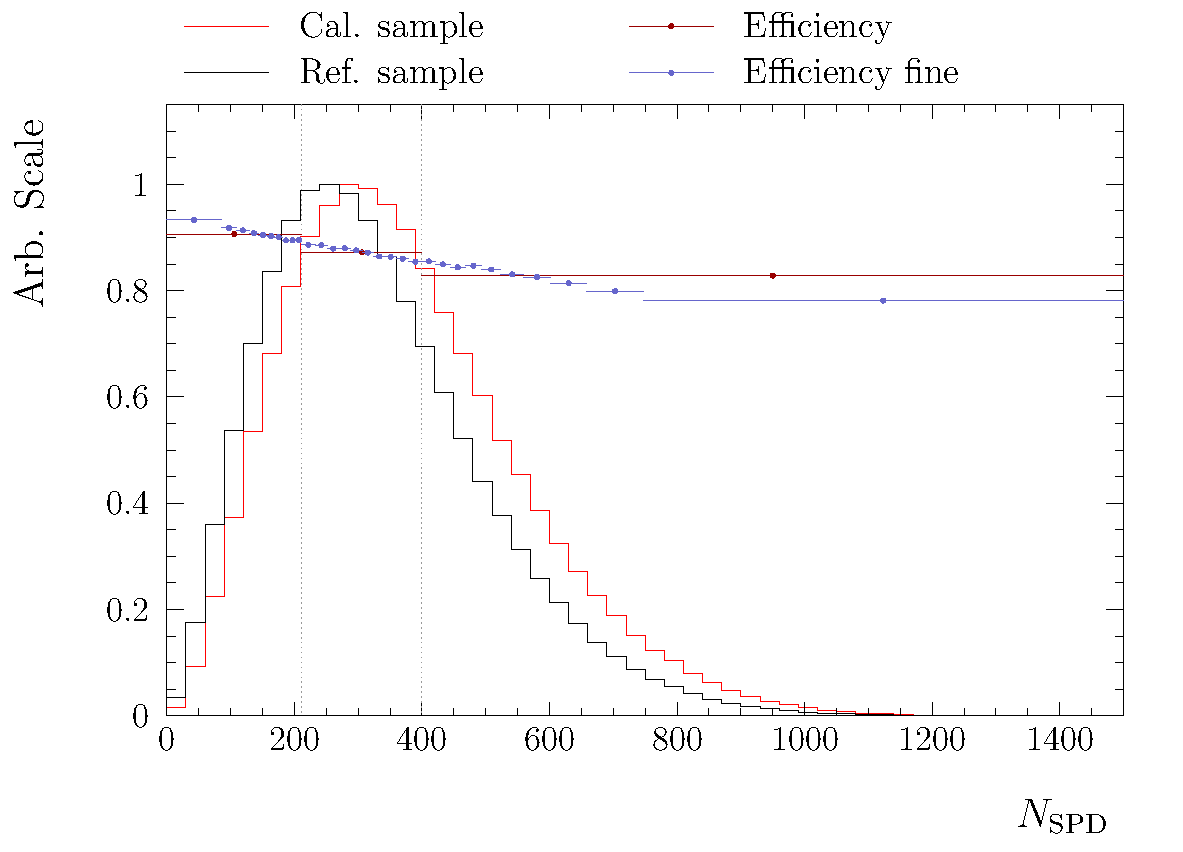
\includegraphics[width=\textwidth,trim={0 0 0 1.75cm},clip]{production/efficiencies/PID_binning_kaon_nspd}
    \caption{\nspd}
    \label{fig:prod:effs:pid:binning:kaon:nspd}
  \end{subfigure}

  \caption{%
    Binning scheme (dark red) used for computing kaon \ac{PID} efficiencies.
    A finer binning scheme (blue) is given to illustrate the varying efficiency
    within the nominal binning scheme.
    The calibration sample distribution (red) and reference sample distribution
    (black) are also shown.
    The distributions are kaon momentum
    (\subref*{fig:prod:effs:pid:binning:kaon:p}) and pseudorapidity
    (\subref*{fig:prod:effs:pid:binning:kaon:eta}) and the event multiplicity
    (\subref*{fig:prod:effs:pid:binning:kaon:nspd}).
  }
  \label{fig:prod:pid:binning:kaon}
\end{figure}

\begin{figure}
  \centering
  \begin{subfigure}[b]{0.7\textwidth}
    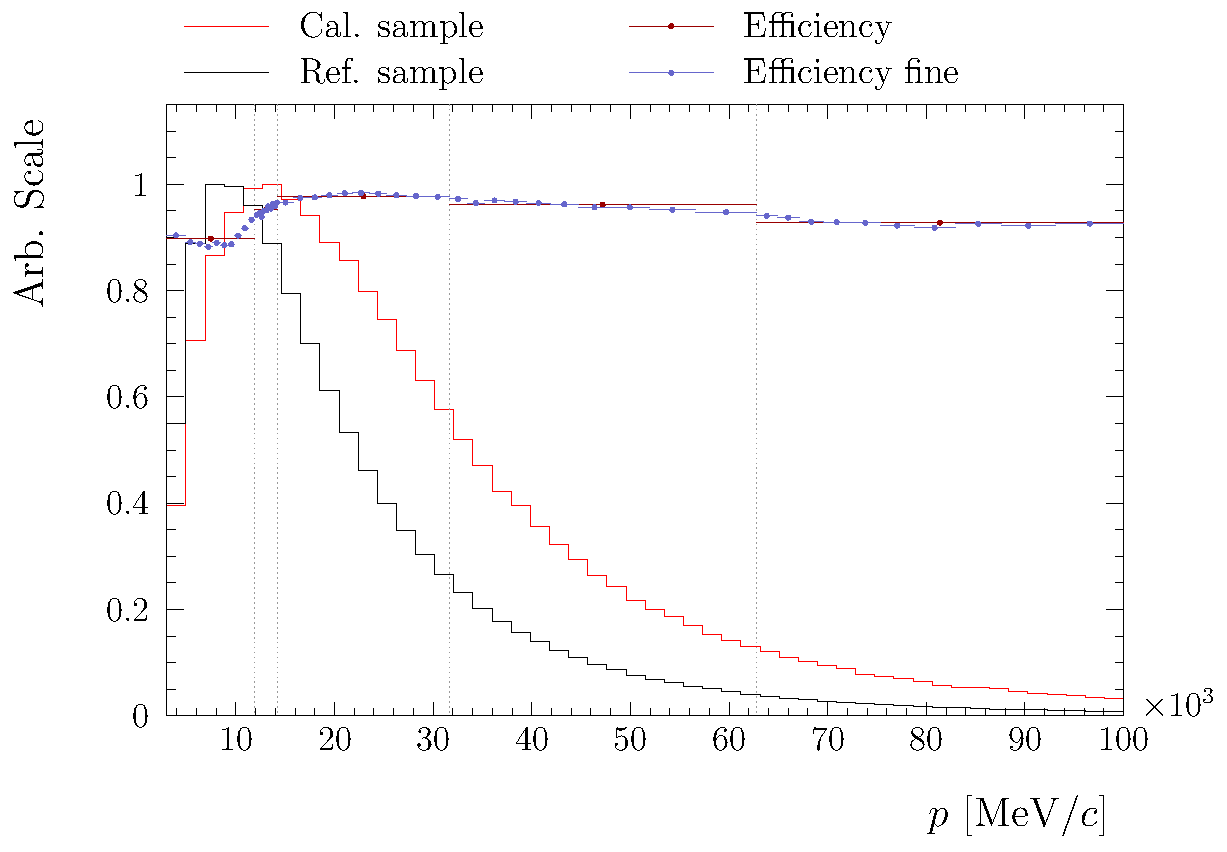
\includegraphics[width=\textwidth,trim={0 0 0 1.75cm},clip]{production/efficiencies/PID_binning_pion_p}
    \caption{Track \ptot}
    \label{fig:prod:effs:pid:binning:pion:p}
  \end{subfigure}
  \begin{subfigure}[b]{0.7\textwidth}
    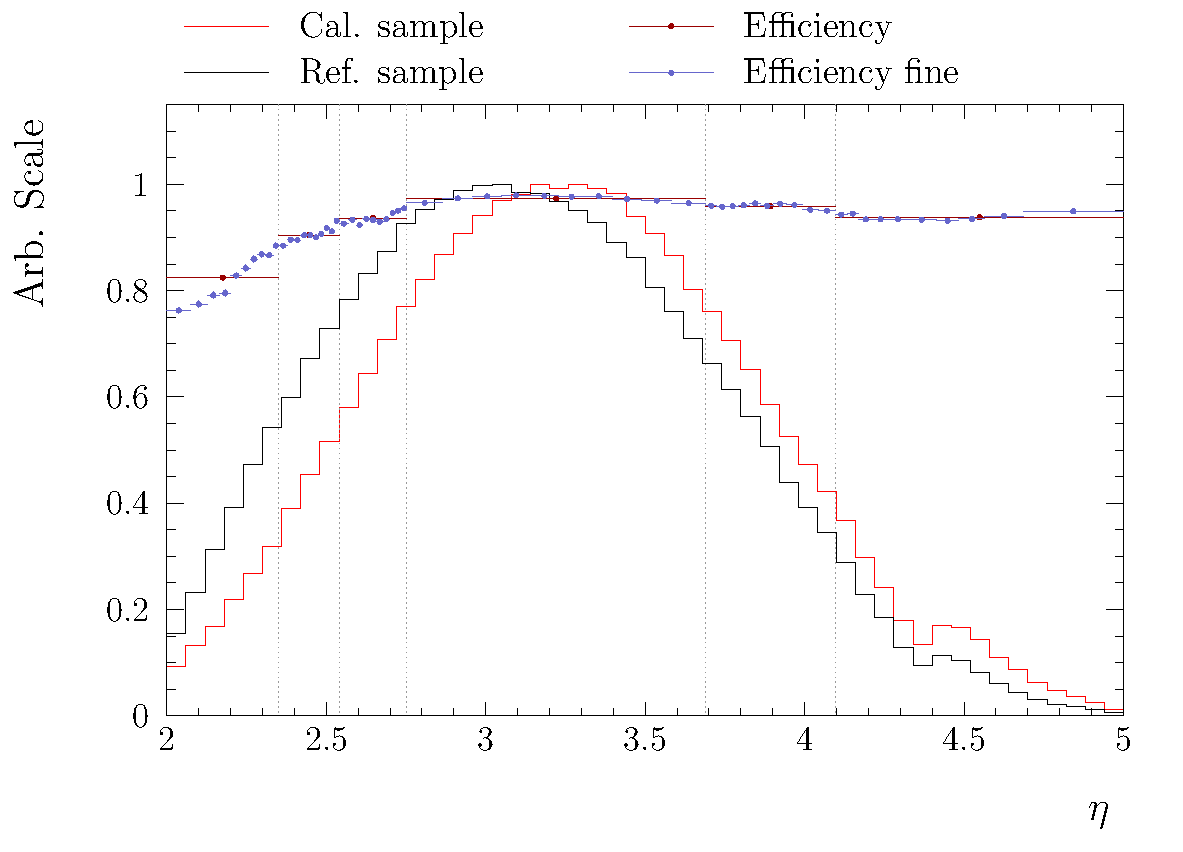
\includegraphics[width=\textwidth,trim={0 0 0 1.75cm},clip]{production/efficiencies/PID_binning_pion_eta}
    \caption{Track \Eta}
    \label{fig:prod:effs:pid:binning:pion:eta}
  \end{subfigure}
  \begin{subfigure}[b]{0.7\textwidth}
    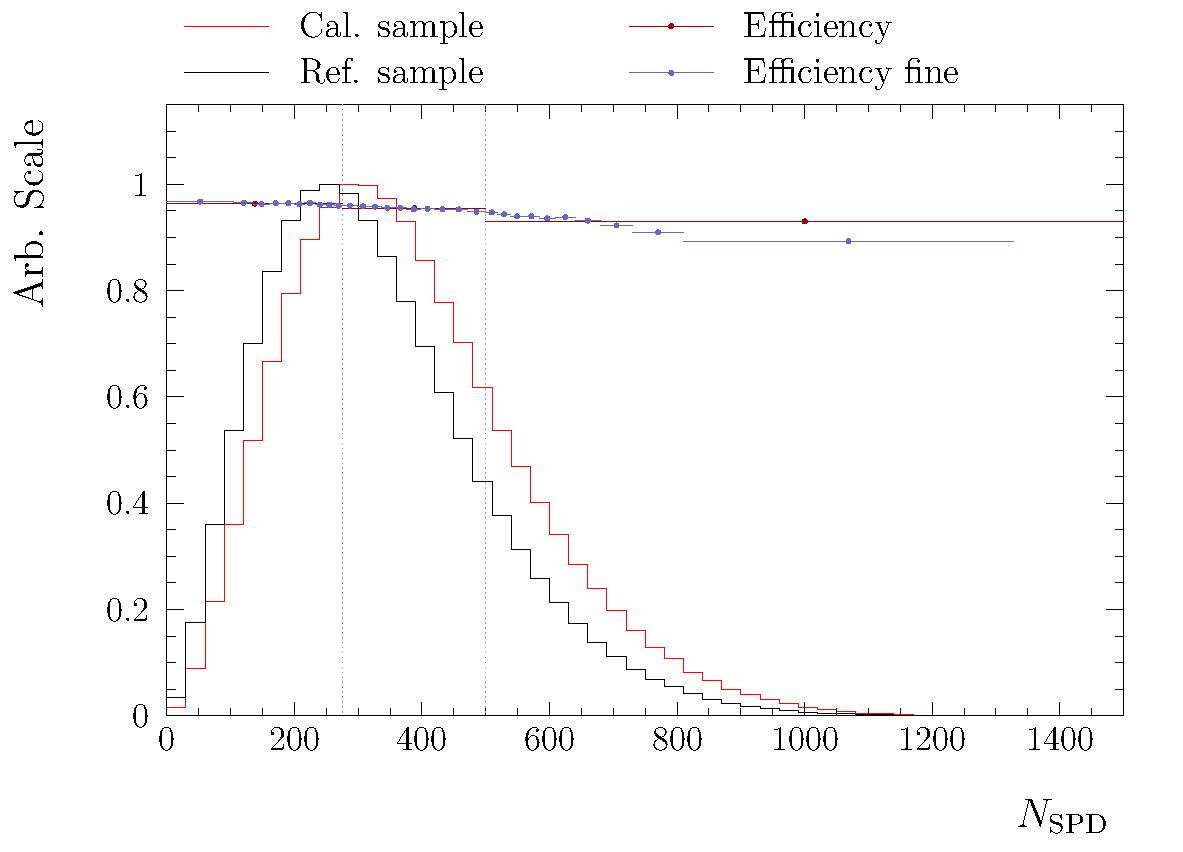
\includegraphics[width=\textwidth,trim={0 0 0 1.75cm},clip]{production/efficiencies/PID_binning_pion_nspd}
    \caption{\nspd}
    \label{fig:prod:effs:pid:binning:pion:nspd}
  \end{subfigure}

  \caption{%
    Binning scheme (dark red) used for computing pion \ac{PID} efficiencies.
    A finer binning scheme (blue) is given to illustrate the varying efficiency
    within the nominal binning scheme.
    The calibration sample distribution (red) and reference sample distribution
    (black) are also shown.
    The distributions are pion momentum
    (\subref*{fig:prod:effs:pid:binning:pion:p}) and pseudorapidity
    (\subref*{fig:prod:effs:pid:binning:pion:eta}) and the event multiplicity
    (\subref*{fig:prod:effs:pid:binning:pion:nspd}).
  }
  \label{fig:prod:pid:binning:pion}
\end{figure}
